
% sizes to get 390 x 286 on dalmatia: -width 382 -height 289
% sizes to get 390 x 286 on sarlat: -width 394 -height 287

\chapter{Rendering}

\section{Overview}

This chapter describes the maspack rendering package ({\tt
maspack.render}), which provides a general interface for the graphical
rendering of objects and allows them to implement their own rendering
methods.  An object makes itself renderable by implementing the
\javaclass[maspack.render]{IsRenderable} interface, and renderable
objects can then be displayed by a \javaclass[maspack.render]{Viewer},
which typically provides features such as viewpoint control, lighting
arrangements, fixtures such as coordinate axes, grids and clipping
planes, and component selection. The viewer also implements a
\javaclass[maspack.render]{Renderer} interface which provides the
actual graphics functionality which renderable objects use to draw
themselves.

\subsection{Renderables and Viewers}
\label{renderersViewers:sec}

Any object to be rendered should implement the
\javaclass[maspack.render]{IsRenderable} interface, which defines the
following four methods,
%
\begin{lstlisting}[]
   void prerender (RenderList list);

   void render (Renderer renderer, int flags);

   void updateBounds (Vector3d pmin, Vector3d pmax);

   int getRenderHints();
\end{lstlisting}
%
\javamethodAlt{maspack.render.IsRenderable.prerender()}{prerender()}
is called prior to rendering and allows the object to update internal
rendering information and possibly give the viewer additional objects
to render by placing them on the
\javaclass[maspack.render]{RenderList} (Section
\ref{prerenderingAndRendering:sec}).
\javamethodAlt{maspack.render.IsRenderable.render()}{render()} is the
main method by which an object renders itself, using the functionality
provided by the supplied \javaclass[maspack.render]{Renderer}.
\javamethodAlt{maspack.render.IsRenderable.updateBounds()}%
{updateBounds()} provides bounds information for the renderable's
spatial extent (which the viewer can use to auto-size the rendering
volume); \javaclass[maspack.matrix]{Vector3d} describes a 3-vector and
is defined in the package {\tt maspack.matrix}.
\javamethod[maspack.render.IsRenderable]{getRenderHints()} returns
flags giving additional information about rendering requirements,
including whether the renderable is transparent
(\javaclassAlt{maspack.render.IsRenderable\#TRANSPARENT}%
{IsRenderable.TRANSPARENT}) or two dimensional
(\javaclassAlt{maspack.render.IsRenderable\#TWO\_DIMENSIONAL}%
{IsRenderable.TWO\_DIMENSIONAL}).
%
\begin{figure}[t]
\begin{center}
\iflatexml
 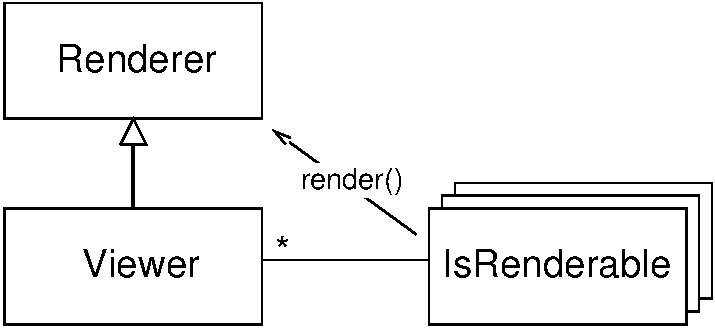
\includegraphics[]{images/viewersRenderables}
\else
 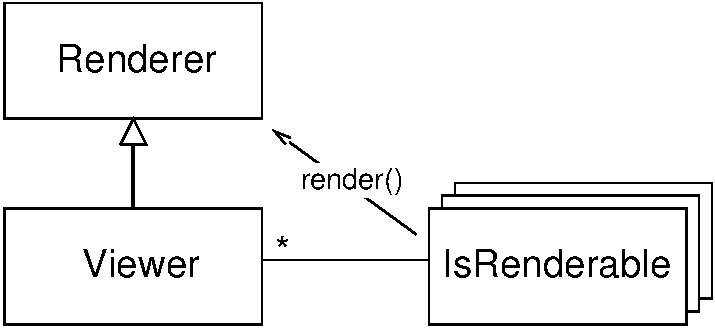
\includegraphics[width=4.00in]{images/viewersRenderables}
\fi
\end{center}
\caption{General relationship between viewers, renderers, and
renderables. A viewer is associated with a number of renderables, and
provides the renderer interface with which renderables use to draw
themselves via their {\tt render()} methods.}
\label{viewersRenderables:fig}
\end{figure}
%

A \javaclass[maspack.render]{Viewer} provides the machinery needed to
display renderable objects, and implements the
\javaclass[maspack.render]{Renderer} interface (Section
\ref{rendererInterface:sec}) with which renderables draw themselves
within their {\tt render()} methods.  {\tt Renderer} includes
methods for maintaining graphics state, drawing primitives such as
points, lines, and triangles, and drawing simple solid shapes.  The
general relationship between viewers, renderables, and renderers is
shown in Figure \ref{viewersRenderables:fig}.  Rendering is triggered
within a viewer by calling its
\javamethod[maspack.render.Viewer]{rerender()} method, which causes
the {\tt prerender()} and {\tt render()} methods to be called for
every renderable, as discussed in detail in Section \ref{viewers:sec}.

%
\begin{figure}[t]
\begin{center}
\iflatexml
 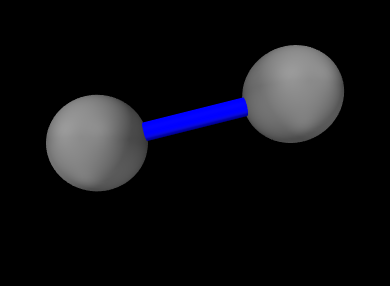
\includegraphics[]{images/renderableExample}
\else
 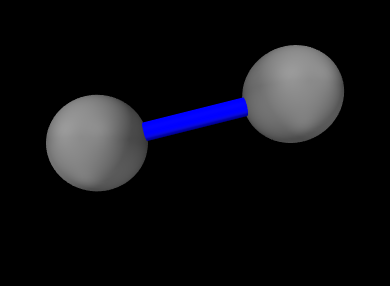
\includegraphics[width=3.75in]{images/renderableExample}
\fi
\end{center}
\caption{Viewer display of the example of Listing \ref{renderableExample:lst}.}
\label{renderableExample:fig}
\end{figure}
%

\subsection{A Complete Example}

Listing \ref{renderableExample:lst} shows a complete example
of a renderable object being declared and displayed in a viewer.
%
\begin{lstlisting}[caption={Declaration and display of a renderable
object.},
label=renderableExample:lst]
package maspack.render;

import java.awt.Color;

import maspack.matrix.Vector3d;
import maspack.matrix.AxisAlignedRotation;
import maspack.render.GL.GLViewerFrame;

public class RenderableExample implements IsRenderable {

   public void prerender (RenderList list) {
      // can be used to cache rendering data or add extra renderables;
      // not used in this example
   }

   public void render (Renderer renderer, int flags) {
      // draw two spheres and a connecting cylinder
      Vector3d pnt0 = new Vector3d (-1, 0, 0);
      Vector3d pnt1 = new Vector3d ( 1, 0.5, 0);
      renderer.setColor (Color.GRAY);
      renderer.drawSphere (pnt0, 0.5);
      renderer.drawSphere (pnt1, 0.5);
      renderer.setColor (Color.BLUE);
      renderer.drawCylinder (pnt0, pnt1, 0.1, /*capped=*/false);
   }

   public void updateBounds (Vector3d pmin, Vector3d pmax) {
      // extend pmin and pmax to accommodate bounds of (-1, -1, 0) and (1, 1, 0)
      (new Vector3d (-1, -1, 0)).updateBoundsz (pmin, pmax);
      (new Vector3d ( 1,  1, 0)).updateBounds (pmin, pmax);
   }

   public int getRenderHints() {
      // no specific hints
      return 0; 
   }

   public static void main (String[] args) {
      IsRenderable renderable = new RenderableExample();
      // create a glviewer in a 640 x 480 frame      
      GLViewerFrame frame = new GLViewerFrame (
         "rendererExample", 640, 480);

      Viewer viewer = frame.getViewer();
      viewer.addRenderable (renderable);
      viewer.setAxialView (AxisAlignedRotation.X_Y); // set view transform
      frame.setVisible (true);
   }
}
\end{lstlisting}
The example creates a class called {\tt RenderableExample} which
implements {\tt isRenderable} and the associated methods: {\tt
prerender()}, which does nothing; {\tt render()}, which draws two gray
spheres connected by a blue cylinder; {\tt updateBounds()}, which sets
the maximum and minimum bounds to be the points $(-1, -1, 0)$ and $(1,
1, 0)$, and {\tt getRenderHints()} which returns no flags. The example
then defines a {\tt main()} method which creates an instance of {\tt
RenderableExample}, along with a {\tt GLViewerFrame} which contains a
viewer with which to display it. The renderable is added to the
viewer, the viewpoint is set so that the $x$ and $y$ axes of the
viewing plane are aligned with the world $x$ and $y$ axes, and the
frame is set to be visible, with the result shown in Figure
\ref{renderableExample:fig}.

\section{Viewers}
\label{viewers:sec}

This section summarizes viewer functionality as defined by the
\javaclass[maspack.render]{Viewer} interface. Note that specific
viewer implementations may provide significant additional
functionality, such as interactive view control, keyboard and mouse
event handling, or graphical fixtures such as coordinate axes, grids
or manipulators. The description of these extra features is beyond the
scope of this document.

Rendering is triggered within a viewer by calling its
\javamethod[maspack.render.Viewer]{rerender()} method, which
then initiates two rendering steps:

\begin{enumerate}

\item {\it prerendering:} The viewer calls the
\javamethod[maspack.render.IsRenderable]{prerender()}
method for all its renderables, and adds those which
are visible into a {\it render list};

\item {\it repainting:} All components in the render list
are redrawn using their
\javamethod[maspack.render.IsRenderable]{render()} method;

\end{enumerate}

Another viewer method, \javamethod[maspack.render.Viewer]{repaint()},
can subsequently be called to initiate repainting {\it without}
invoking prerendering.  

In general, {\tt rerender()} should be called whenever there is a
change in the graphical state of the renderables. This includes
changes in geometry, color, or visibility.  In the context of
simulation, {\tt rerender()} should be called after every simulation
step.

Otherwise, {\tt repaint()} should be called when the graphical state
of the scene has not changed but the final screen display has, such as
when the viewpoint is changed, or the display window is unhidden or
resized. This is more efficient than calling {\tt rerender()} because
it avoids the overhead of the prerendering step.

The prerendering step is invoked directly within the {\tt rerender()}
method, whereas the repainting step is called in whatever thread
implements the graphical display. Since, as described below, one of
the functions of the prerendering step is to cache rendering
information, {\tt rerender()} should be called in synchronization with both the
graphical display thread and whatever thread(s) (such as a simulation
thread) might be altering the state of the renderables.

\subsection{Render lists}
\label{RenderLists:sec}

A {\it render list} is implemented by the class
\javaclass[maspack.render]{RenderList} and sorts renderable components
into separate sublists depending on whether they are primarily {\it
opaque}, {\it transparent}, {\it 2d opaque}, and {\it 2d transparent}.
These designations are determined by examining the flags returned by
the renderable's
\javamethod[maspack.render.IsRenderable]{getRenderHints()} method,
with {\tt TWO\_DIMENSIONAL} indicating a two dimensional component and
{\tt TRANSPARENT} indicating a transparent one. These sublists assist
the viewer in rendering a scene more realistically.  For example, in
OpenGL, better results are obtained if opaque objects are drawn before
transparent ones, and two dimensional objects are drawn after three
dimensional ones, with the depth buffer disabled.

A viewer maintains its own internal render list, and rebuilds it once
during every prerendering step, using the following algorithm:
%
\begin{lstlisting}[]
RenderList list;
for (each renderable component r) {
   list.addIfVisible (r);
}
\end{lstlisting}
%
The list's \javamethod[maspack.render.RenderList]{addIfVisible()}
method calls the component's {\tt prerender()} method, and then adds
it to the appropriate sublist if it is visible:
%
\begin{lstlisting}
addIfVisible (IsRenderable r) {
   r.prerender();
   if (r is visible) {
      add r to appropriate sublist;
   }
}
\end{lstlisting}
%
A renderable's visibility is determined as follows:

\begin{itemize}

\item Any object implementing \javaclass[maspack.render]{IsRenderable}
is visible by default.

\item If the object also implements
\javaclass[maspack.render]{HasRenderProps} (as described in Section
\ref{RenderProps:sec}), then it is visible only if
the \javaclass[maspack.render]{RenderProps} returned by
\javamethod[maspack.render.HasRenderProps]{getRenderProps()} is
non-null and the associated {\sf visible} property is {\tt true}.

\end{itemize}

As discussed in Section \ref{viewerRenderables:sec}, a viewer can also
be provided with an {\it external render list}, which is maintained by
the application. It is the responsbility of the application, and not
the viewer, to rebuild the external render list during the
prerendering step. However, in the repainting step, the viewer will
handle the redrawing of all the components in both its internal and
external render lists.

\subsection{Prerendering and Rendering}
\label{prerenderingAndRendering:sec}

Prerendering allows renderables to

\begin{enumerate}

\item update data structures anc cached data needed for rendering

\item add additional renderables to the render list.

\end{enumerate}

The caching of graphical state is typically necessary when rendering
is performed in a thread separate from the main application, which can
otherwise cause synchronization and consistency problems for
renderables which are changing dynamically. For example, suppose we
are simulating the motion of two objects, A and B, and we wish to
render their positions at a particular time t. If the render thread is
allowed to run in parallel with the thread computing the simulation,
then A and B might be drawn with positions corresponding to different
times (or worse, positions which are indeterminate!).

Synchronizing the rendering and simulation threads will aleviate this
problem, but that means foregoing the speed improvement of allowing
the rendering to run in parallel. Instead, renderables can use the
{\tt prerender()} method to cache their current state for later use in
the {\tt render()} method, in a manner analagous to double buffering.
For example, suppose a renderable describes the position of a point in
space, inside a member variable called {\tt myPos}. Then its {\tt
prerender()} method can be constructed to save this into
another another member variable {\tt myRenderPos} for later use in
{\tt render()}:
%
\begin{lstlisting}[]
import maspack.geometry.Vector3d;
import maspack.render.*;
...

   Vector3d myPos;         // point position
   float[] myRenderPos;   // cached value for rendering

   void prerender (RenderList list) {
      ...
      myPos.get (myRenderPos); // save cached value
      ...
   }
\end{lstlisting}
%
In the example above, the cached value is stored using floating point
values, since this saves space and usually provides sufficient
precision for rendering purposes.

As described in Section \ref{renderObjects:sec}, objects can sometimes
make use of {\it render objects} when rendering themselves. These can
result in improved graphical efficieny, and also provide an alternate
means for caching graphical information. If render objects are being
used, it is recommmended that they be created or updated within {\tt
prerender()}.

The {\tt prerender()} method can also be used to add additional
renderables to the render list. This is done by recursively calling
the list's \javamethod[maspack.render.RenderList]{addIfVisible()}
method.
For example, if a
renderable has two subcomponents, A and B, which also need to 
be rendered, then it can add them to the render list as follows:
\begin{lstlisting}[]
void prerender (RenderList list) {
   IsRenderable A, B;

   ... 
   // add both A and B to the render list
   list.addIfVisible (A);
   list.addIfVisible (B);
}
\end{lstlisting}
In addition to adding A and B to the render list if they are visible,
{\tt addIfVisible()} will also call their {\tt prerender()} methods,
which will in turn give them the opportunity to add their own sub
components to the render list. Note that {\tt prerender()} is always
called for the specified renderable, whether it is visible (and added
to the list) or not (since even if a renderable is not visible, it
might have subcomponents which are).  This allows an entire hierarchy
of renderables to be rendered by simply adding the root renderable to
the viewer.

Note that any renderables added to the render list within {\tt
prerender()} are {\bf not} added to the primary list of renderables
maintained by the viewer.

\begin{sideblock}
Because of the functionality outlined above, calls to {\tt
prerender()} methods, and the viewer {\tt rerender()} method that
invokes them, should be synchronized with both the graphical display
thread and whatever thread(s) might be altering the state of the
renderables.
\end{sideblock}

As indicated above, actual object rendering is done within its {\tt
render()} method, which is called during the repaint step, within
whatever thread is responsible for graphical display.  The {\tt
render()} method signature,
%
\begin{lstlisting}[]
void render (Renderer renderer, int flags)
\end{lstlisting}
%
provides a \javaclass[maspack.render]{Renderer} interface (Section
\ref{rendererInterface:sec}) which the object uses to draws itself,
along with a {\tt flags} argument that specifies additional rendering
conditions.  Currently only one flag is formally supported,
\javaclassAlt{maspack.render.Renderer\#HIGHLIGHT}% 
{Renderer.HIGHLIGHT},
which requests that the object be rendered using
highlighting (see Section \ref{highlighting:sec}).

\subsection{Viewer renderables and external render lists}
\label{viewerRenderables:sec}

Renderables can be added or removed from a viewer using the methods
\begin{lstlisting}[]
   void addRenderable (IsRenderable r);
   void removeRenderale (IsRenderable r);
   void clearRenderables();
\end{lstlisting}

If renderables are arranged in a hierarchy, and add their own
subcomponents to the render list during {\tt prerender()}, as
described in Section \ref{prerenderingAndRendering:sec}, then it may
only be necessary to add top level renderable components to the
viewer.

It is also possible to assign a viewer an {\it external render list},
for which the prerendering step is maintained by the application. This
is useful in situations where multiple viewers are being used to
simultaneously render a common set of renderables. In such cases, it
would be wasteful for each viewer to repeatedly execute the prerender
phase on the same renderable set. It may also lead to inconsistent
results, if the state of renderables changes between different viewers'
invocation of the prerender phase.

To avoid this problem, an application may create its own render list
and then give it to multiple viewers using
\javamethod[maspack.render.Viewer]{setExternalRenderList()}.
A code sample for this is as follows:
\begin{lstlisting}[]
import maspack.render.*;
...

   Viewer viewer1;
   Viewer viewer2;
   List<IsRenderable> renderables;

   RenderList extlist = new RenderList();

   // assign external list to the viewers
   viewer1.setExternalRenderList (extlist);
   viewer2.setExternalRenderList (extlist);

   for (each simulation step) {

      // execute the pre-render phase
      syncrhonized (extlist) {
         for (IsRenderable r : renderables) {
            extlist.addIfVisibleAll (r);
         }
      }
      viewer1.rerender();
      viewer2.rerender();
   }
\end{lstlisting}
The statement {\tt synchronize(extlist)} ensures that calls to {\tt
extlist.addIfVisible(r)} (and the subsequent internal calls to {\tt
prerender()}) are synchronized with {\tt render()} method calls made by
the viewer. This works because the viewer also wraps its usage of 
{\tt extlist} inside {\tt synchronize(extlist)} statements.

Once the viewers have been assigned an external render list, they will
handle the repainting step for its renderables, along with their own
internal renderables, every time repainting is invoked through a call
to either \javamethod[maspack.render.Viewer]{rerender()} (as in the
above example) or \javamethod[maspack.render.Viewer]{repaint()}.

\subsection{Coordinate frames and view point control}
\label{coordinateFrames:sec}

A viewer maintains three primary coordinate frames for describing the
relative locations and orientations of scene objects and the observing
``eye'' (or camera). These are the {\it eye}, {\it model}, and {\it
world} frames.

The {\it eye frame} (sometimes also known as the camera frame) is a
right-handed frame located at the eye (or camera) focal point, with
the $z$ axis pointing toward the observer. The {\it viewing frustum}
is located in the half space associated with the negative $z$ axis of
the eye frame (and usually centered on said axis), with the near and
far clipping planes designated as the {\it view plane} and {\it far
plane}, respectively. The viewer also maintains a viewing {\it
center}, typically located along the negative $z$ axis, and which
defines the point about which the camera pivots in response to
interactive view rotation.

The viewing frustum is defined by the view and far planes, in
combination with a projection matrix that transforms eye coordinates
into clip coordinates. Most commonly, the projection matrix is set up
for perspective viewing (Figure \ref{coordinateFrames:fig}), but
orthographic viewing (Figure \ref{orthographic:fig}) is sometimes used as
well.

%
\begin{figure}[t]
\begin{center}
\iflatexml
 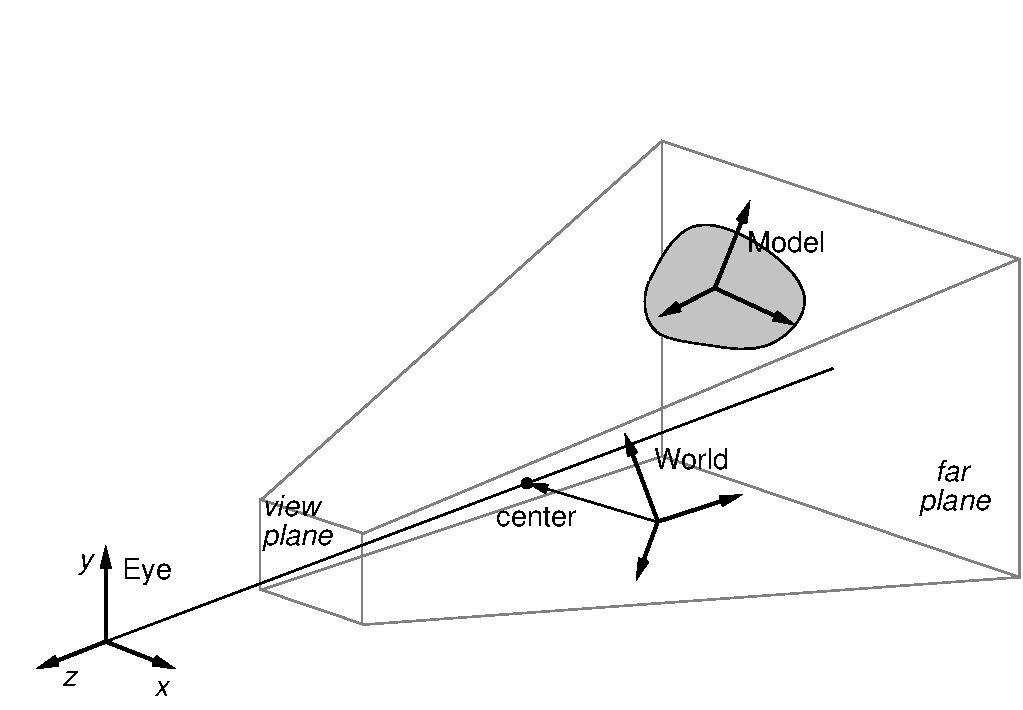
\includegraphics[]{images/coordinateFrames}
\else
 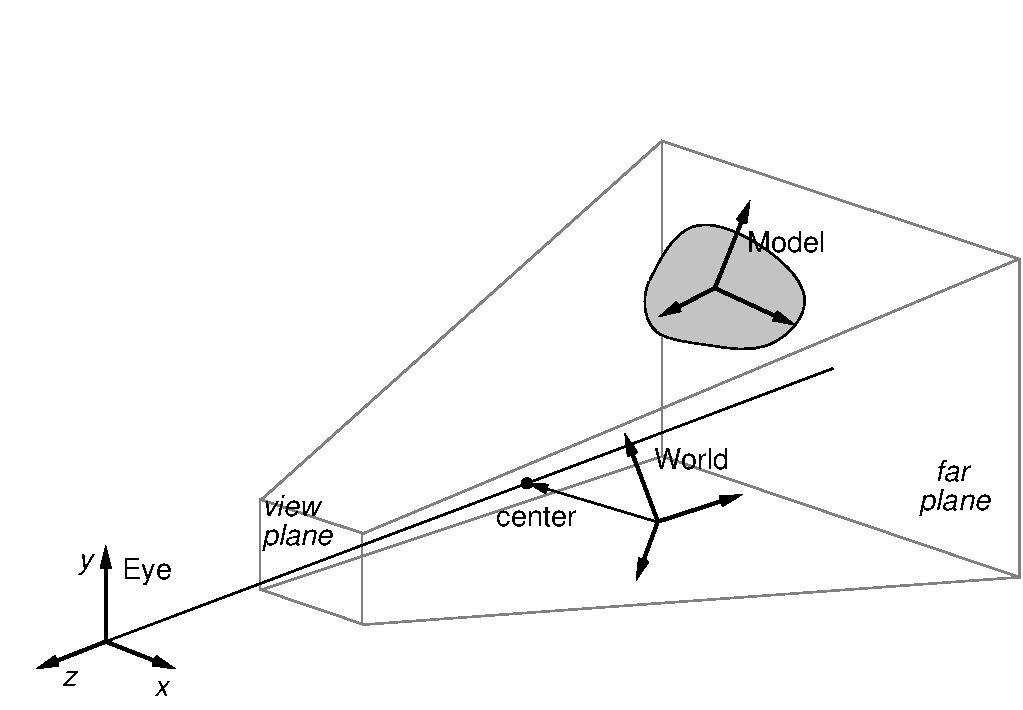
\includegraphics[width=5.5in]{images/coordinateFrames}
\fi
\end{center}
\caption{Primary coordinate frames associated with the renderer, along with
the viewing frustum and center point.}
\label{coordinateFrames:fig}
\end{figure}
%

%
\begin{figure}[t]
\begin{center}
\iflatexml
 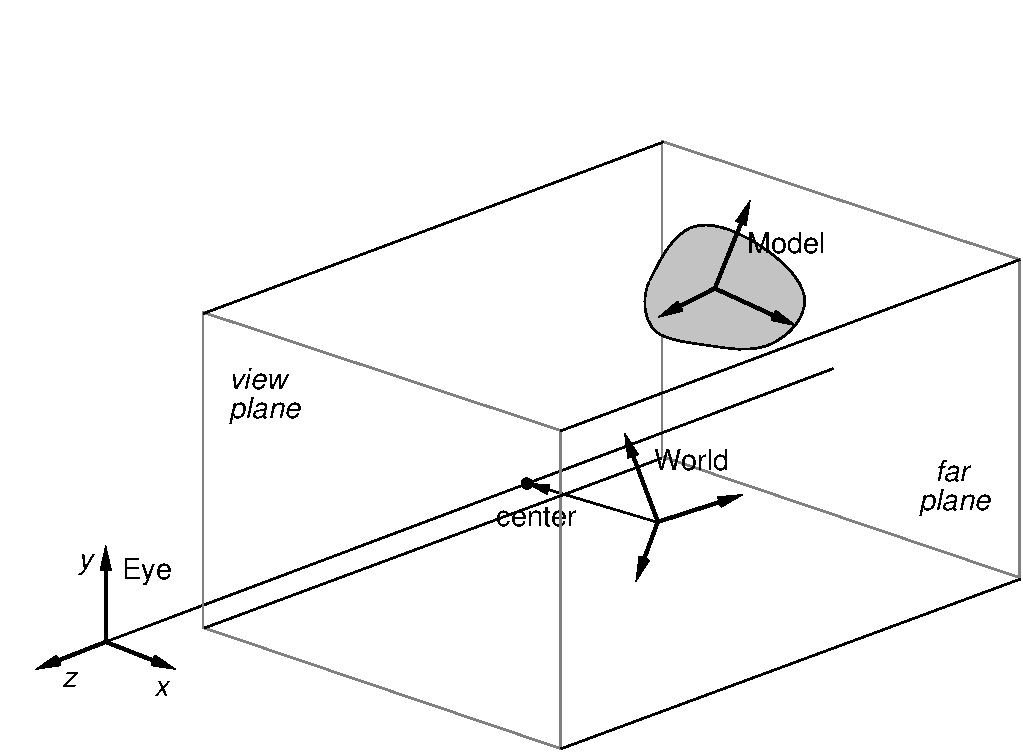
\includegraphics[]{images/orthographic}
\else
 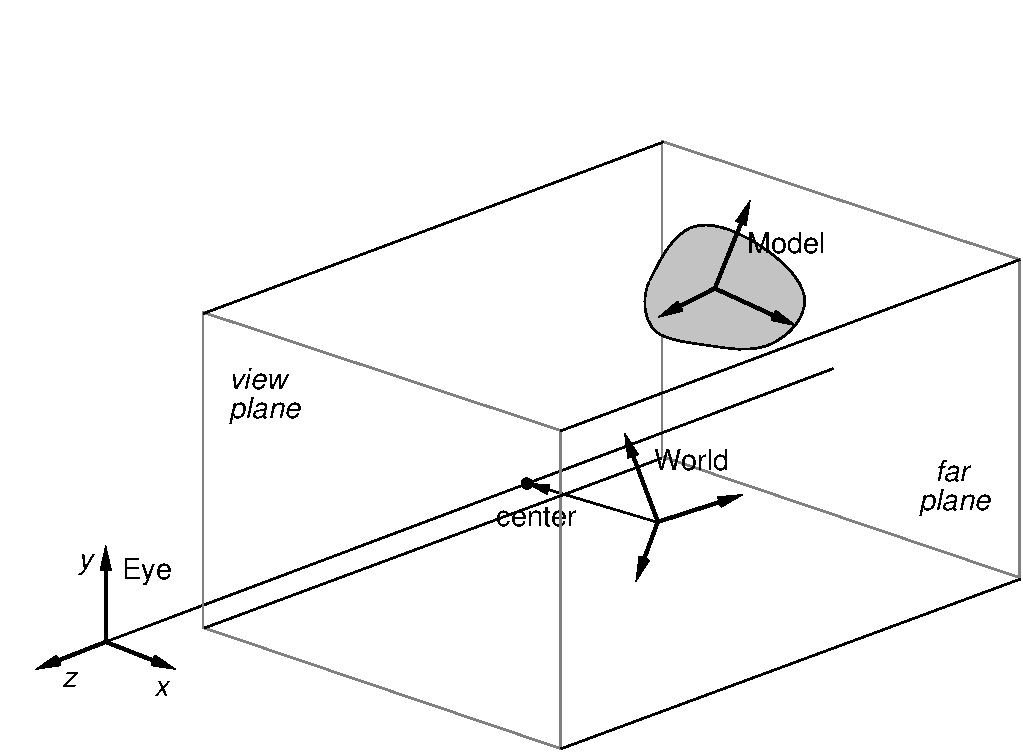
\includegraphics[width=5.5in]{images/orthographic}
\fi
\end{center}
\caption{Primary coordinate frames with the projection matrix set up
for orthographic viewing.}
\label{orthographic:fig}
\end{figure}
%

The {\it model frame} is the coordinate frame in which geometric
information for rendered objects is specified, and the {\it world frame} is the
base with respect to which the model and eye frames are defined. The
{\it model matrix} is the $4 \times 4$ homogeneous affine transform
$\X_{MW}$ from model to world coordinates, while the {\it view matrix}
is a $4 \times 4$ homogeneous rigid transform $\T_{WE}$ from world to eye
coordinates. The composition of $\T_{WE}$ and $\X_{MW}$ transforms a
point from model coordinates ${}^M\p$ into eye coordinates ${}^E\p$,
according to:
%
\begin{equation*}
\matl {}^E\p \\ 1 \matr \;=\;
\T_{WE} \, \X_{MW} \matl {}^M\p \\ 1 \matr.
\end{equation*}
%

\begin{sideblock}
Note: the renderer assumes that points and vectors are column-based
and the coordinate transforms work by pre-multiplying these column
vectors. This is in constrast to some computer graphics conventions in
which vectors are row based. Our transformation matrices are therefore
the transpose of those defined with respect to a row-based convention.
\end{sideblock}

Initially the world and model frames are coincident, so that $\X_{MW}
= \I$. Rendering methods often redefine the model matrix, allowing
existing object geometry or built-in drawing methods to be used at
different scales and poses throughout the scene.  The methods
available for querying and controlling the model matrix are described
in Section \ref{modelMatrix:sec}.

%
\begin{figure}[t]
\begin{center}
\iflatexml
 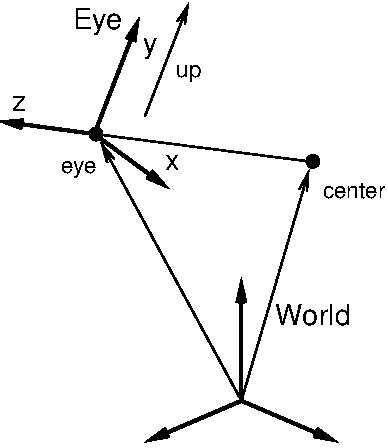
\includegraphics[]{images/eyeCenterUp}
\else
 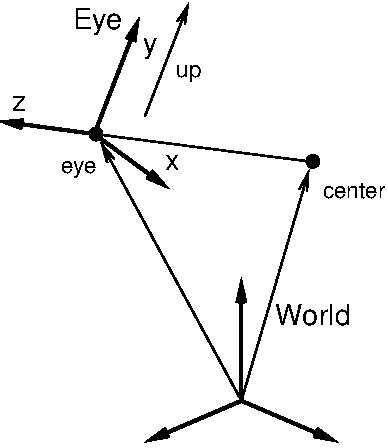
\includegraphics[width=2.5in]{images/eyeCenterUp}
\fi
\end{center}
\caption{Determining the pose of the eye frame from the {\tt eye} and
{\tt center} points, and an {\tt up} vector parallel to the frame's
$y$ axis.}
\label{eyeCenterUp:fig}
\end{figure}
%
Meanwhile, changing the view matrix allows the scene to be
observed from different view points. A viewer provides the following
direct methods for setting and querying the view matrix:
%
\begin{lstlisting}[]
void setViewMatrix (RigidTransform3d TWE);
RigidTransform3d getViewMatrix();
void getViewMatrix (RigidTransform3d TWE);
\end{lstlisting}
%
where 
\javaclass[maspack.matrix]{RigidTransform3d} is defined
in {\tt maspack.matrix} and represents a $4 \time 4$ homogenous
rigid transformation.
Instead of specifying the view matrix, it is sometimes more convenient
to specify its inverse, the eye-to-world transform $\T_{EW}$.
This can be done with
%
\begin{lstlisting}[]
void setEyeToWorld (RigidTransform3d TEW);
void setEyeToWorld (Point3d eye, Point3d center, Vector3d up);
void getEyeToWorld (RigidTransform3d TEW);
\end{lstlisting}
%
where 
\javaclass[maspack.matrix]{Point3d} and
\javaclass[maspack.matrix]{Vector3d} are also defined in 
{\tt maspack.matrix} and represent 3 dimensional points and vectors.
The method
\javamethodAlt{maspack.render.Viewer.setEyeToWorld(Point3d,Point3d,Vector3d)}%
{setEyeToWorld(eye,center,up)} sets $\T_{EW}$ according to legacy
OpenGL conventions so that (with respect to world coordinates) the eye
frame's origin is defined by the point {\tt eye}, while its
orientation is defined such that the $-z$ axis points from {\tt eye}
to {\tt center} and the $y$ axis is parallel to {\tt up} (see Figure
\ref{eyeCenterUp:fig}).

\begin{sideblock}
\javaclass[maspack.matrix]{Point3d} is a subclass of
\javaclass[maspack.matrix]{Vector3d} used to describe points in
space. The only difference between the two is that they transform
differently in response to rigid transforms (described by
\javaclass[maspack.matrix]{RigidTransform3d}) or affine transforms
(described by \javaclass[maspack.matrix]{AffineTransform3d}): point
transformations include the translational component, while vector
transformations do not.
\end{sideblock}

The viewer also maintains a {\tt center} position and an {\tt up}
vector that are used to modify $\T_{EW}$ in conjunction
with the following:
%
\begin{lstlisting}[]
void setEye (Point3d eye);
Point3d getEye();

void setCenter (Point3d center);
Point3d getCenter();

void setUpVector (Vector3d up);
Vector3d getUpVector();
\end{lstlisting}
%
Again with respect to world coordinates,
\javamethodAlt{maspack.render.Viewer.setEye(Point3d)}{setEye(eye)}
sets the origin of the eye frame while recomputing its orientation
from the current values of {\tt center} and {\tt up}, while
\javamethodAlt{maspack.render.Viewer.setCenter(Point3d)}{setCenter(center)}
and
\javamethodAlt{maspack.render.Viewer.setUpVector()}{setUpVector(up)}
set {\tt center} and {\tt up} and recompute the eye frame's
orientation accordingly.

It is also possible to specify axis-aligned views, so that the axes of
the eye frame are exactly aligned with the axes of the world
frame. This can be done using
%
\begin{lstlisting}[]
void setAxialView (AxisAlignedRotation REW);
AxisAlignedRotation getAxialView();
\end{lstlisting}
%
\javamethod[maspack.render.Viewer]{setAxialView()} sets the rotational
component of $\T_{EW}$ to {\tt REW}, and moves the eye position so
that the viewer's {\tt center} lies along the new $-z$ axis. It also
sets the {\tt up} vector to the $y$ axis of {\tt REW}, and stores {\tt
REW} as the viewer's nominal {\it axial view} which can be used for
determining default orientations for fixtures such as grids.
\javaclass[maspack.matrix]{AxisAlignedRotation} defines 24 possible
axis-aligned orientations, and so there are 24 possible axis-aligned
views. Some of those commonly used in association with {\tt
setAxialView()} are:

\begin{center}
\begin{tabular}{|l|l|}
\hline 
X\_Y & eye frame and world frame have the same orientaion\\
X\_Z & eye frame $x$-$y$ axes correspond to world frame $x$-$z$\\
Y\_Z & eye frame $x$-$y$ axes correspond to world frame $y$-$z$\\
\hline
\end{tabular}
\end{center}

There are several methods available to reset the viewing frustum:
%
\begin{lstlisting}[]
void setPerspective (
   double left, double right, double bottom, double top, double near, double far);
void setPerspective (
   double fieldOfView, double near, double far);

void setOrthogonal (
   double left, double right, double bottom, double top, double near, double far);
void setOrthogonal (
   double fieldHeight, double near, double far);
\end{lstlisting}
%
The {\tt setPerspective} methods create a perspective-based frustum
(Figure \ref{coordinateFrames:fig}). The first methods explicitly sets
the left, right, bottom and top edges of the view plane, along with
the (positive) distances to the near (i.e., view) and far planes,
while the second method creates a frustum centered on the $-z$ axis,
using a specified vertical field of view. The {\tt setOrthogonal}
methods create an orthographic frustum (Figure \ref{orthographic:fig})
in a similar manner.

Information about the current frustum can be queried using
%
\begin{lstlisting}[]
double getViewPlaneWidth();
double getViewPlaneHeight();
double getViewPlaneDistance();
double getFarPlaneDistance();

Vector3d getEyeZDirection();
boolean isOrthogonal();
\end{lstlisting}
%

For convenience, the viewer can also automatically determine
appropriate values for the {\tt center} and {\tt eye} positions, and
then fit a suitable viewing frustum around the scene. This is done
using the renderables'
\javamethod[maspack.render.IsRenderable]{updateBounds()} method to
estimate a scene center and radius, along with the current value of
the {\tt up} vector to orient the eye frame. The auto-fitting
methods are:
%
\begin{lstlisting}[]
void autoFitOrtho();        // fit orthographic frustum
void autoFitPerspective();  // fit perspective frustum
void autoFit();             // fit frustum of the current type
\end{lstlisting}
%
These auto-fit methods also make use of a default vertical
field-of-view, which is initially 35 degrees and which
can be controlled using
%
\begin{lstlisting}[]
double getVerticalFieldOfView();
void setVerticalFieldOfView (double fov);
\end{lstlisting}
%

Finally, the viewer's background color can be controlled using
%
\begin{lstlisting}[]
void setBackgroundColor (float[] rgba)
void setBackgroundColor (Color color);
Color getBackgroundColor();
float[] getBackgroundColor(float[] rgba);
\end{lstlisting}
%

\subsection{Lights}
\label{lights:sec}

Viewers also maintain scene lighting. Typically, a viewer will be
initialized to a default set of lights, which can then be
adjusted by the application. The existing
light set can be queried using the methods
%
\begin{lstlisting}[]
   int numLights();                   // number of lights currently in use
   Light getLight (int idx);          // get information for the idx-th light 
   int getIndexOfLight (Light light); // return index for light, or -1
\end{lstlisting}
%
where \javaclass[maspack.render]{Light} is a class 
containing parameters for the light.
Lights are described using the same parameters as those of OpenGL,
as described in Chapter 5 of the OpenGL Programming Guide (Red book).
Each has a position $\p$ and (unit) direction $\bf d$ in space, a {\it
type}, colors associated with ambient, specular and diffuse lighting,
and coefficients for its attenuation formula. The attenuation formula
is
%
\begin{equation*}
f = \frac{1}{C + L d + D d^2}
\end{equation*}
%
where $f$ is the light intensity, $d$ is the distance between the
light and the point being lit, and $C$, $L$, and $D$ are the constant,
linear and quadratic attentuation factors. 

Spot lights have the same properties as other lights, in addition to
also having a {\it cutoff angle} $\theta$ and an {\it exponent} $e$.
The cutoff angle is the angle between the direction of the light and
the edge of its cone, while the exponent, whose default value is 0, is
used to determine how focused the light is. If $\bf{v}$ is the unit
direction from the light to the point being lit, and if $ {\bf d}
\cdot {\bf v} \ge \cos \theta $, then the point being lit is within
the light cone and the light intensity $f$ in the above equation is
multiplied by the {\it spotlight effect}, given by
%
\begin{equation*}
({\bf d} \cdot {\bf v})^e
\end{equation*}
%
Since $ |{\bf d} \cdot {\bf v}| \le 1$, a value of $e = 0$ gives
the least light reductuon, while valuse of $e > 0$ increase the
intensity of the spot light towards its center.

Information for a specific light is provided by a
\javaclass[maspack.render]{Light} object, which contains the following
fields:

\begin{description}

\item[enabled]\mbox{}

A boolean describing whether or not the light is enabled.

\item[type]\mbox{}

An instance of \javaclass[maspack.render]{Light\$LightType}
describing the type of the light. Current values are
{\tt DIRECTIONAL}, {\tt POINT}, and {\tt SPOT}.

\item[position]\mbox{}

A 3-vector giving the position of the light in world coordinates.

\item[direction]\mbox{}

A 3-vector giving the direction of the light in world coordinates.

\item[ambient]\mbox{}

RGBA values for the ambient light color.

\item[diffuse]\mbox{}

RGBA values for the diffuse light color.

\item[specular]\mbox{}

RGBA values for the specular light color.

\item[constantAttenuation]\mbox{}

Constant term C in the attenuation formula

\item[linearAttenuation]\mbox{}

Linear term L in the attenuation formula

\item[quadraticAttenuation]\mbox{}

Quadratic term Q in the attenuation formula

\item[spotCosCutoff]\mbox{}

For spotlights, the cosine of the cutoff angle $\theta$.

\item[spotExponent]\mbox{}

For spotlights, the exponent $e$.

\end{description}

Each of these fields is associated with accessor methods inside
\javaclass[maspack.render]{Light}.

An application can also add or remove lights using
%
\begin{lstlisting}[]
void addLight (Light light);
boolean removeLight (Light light)
boolean removeLight (int idx);
\end{lstlisting}
%
To create a new light, the application instantiates a {\tt Light}
object, sets the appropriate fields, and then calls
\javamethod[maspack.render.Viewer]{addLight()}. Lights can be
removed either by reference to the light object or its index.

\begin{sideblock}
Lights are updated by the viewer at the beginning of each repaint
step. That means that for lights already added to the viewer, any
changes made to the fields of the associated
\javaclass[maspack.render]{Light} object will take effect
at the beginning of the next repaint step.
\end{sideblock}

\section{The Renderer Interface}
\label{rendererInterface:sec}

This section describes the \javaclass[maspack.render]{Renderer}
interface, which supplies the methods which objects can use to draw
themselves. This includes methods for setting graphics state, and
drawing point, line and triangle primitives as well as simple solid
shapes.

\subsection{Drawing single points and lines}
\label{singlePointsLines:sec}

The most basic Renderer methods provide for the drawing of single
points, lines, and triangles. The following can be used to
draw a pixel-based point at a specified location {\tt pnt}, or a
pixel-based line segment between two points {\tt pnt0} and {\tt pnt1}:
%
\begin{lstlisting}[]
void drawPoint (Vector3d pnt);
void drawPoint (double px, double py, double pz);
void drawPoint (float[] pnt);

void drawLine (Vector3d pnt0, Vector3d pnt1);
void drawLine (double px0, double py0, double pz0, 
               double px1, double py1, double pz1);
void drawLine (float[] pnt0, float[] pnt1);
\end{lstlisting}
%
where, as mentioned earlier, \javaclass[maspack.matrix]{Vector3d} 
represents a 3-vector and is defined in {\tt maspack.matrix}.
\begin{sideblock}
Note: while convenient for drawing small numbers of points and lines,
the methods described in this section can be quite inefficient. For
rendering larger numbers of primitives, one should use either the {\it
draw mode} methods of Section \ref{drawMode:sec}, or the even more
efficient {\it render objects} described in Section
\ref{renderObjects:sec}.
\end{sideblock}

The size of the points or lines (in pixels) can be controlled via
following methods:
%
\begin{lstlisting}[]
float getPointSize();
void setPointSize(float size);

float getLineWidth();
void setLineWidth (float width);
\end{lstlisting}
%
\begin{figure}[t]
\begin{center}
\iflatexml
 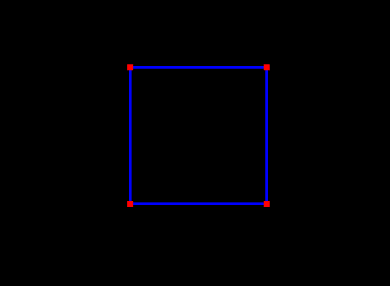
\includegraphics[]{images/drawSquare}
\else
 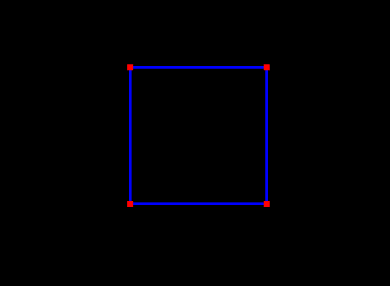
\includegraphics[width=3.75in]{images/drawSquare}
\fi
\end{center}
\caption{Simple square drawn with the renderer.}
\label{drawSquare:fig}
\end{figure}
%
The following example draws a square in the x-z plane, with blue edges
and red corners:
%
\begin{lstlisting}[]
import java.awt.Color;
import maspack.matrix.Vector3d;
import maspack.render.*;
import maspack.render.Renderer.Shading;
...

   void render (Renderer renderer, int flags) {
   
      // the corners of the square
      Vector3d p0 = new Vector3d (0, 0, 0);
      Vector3d p1 = new Vector3d (1, 0, 0);
      Vector3d p2 = new Vector3d (1, 0, 1);
      Vector3d p3 = new Vector3d (0, 0, 1);
   
      renderer.setShading (Shading.NONE); // turn off lighting
   
      // draw corners
      renderer.setPointSize (4);
      renderer.setColor (Color.RED);
      renderer.drawPoint (p0);
      renderer.drawPoint (p1);
      renderer.drawPoint (p2);
      renderer.drawPoint (p3);
   
      // draw edges
      renderer.setLineWidth (2);
      renderer.setColor (Color.BLUE);
      renderer.drawLine (p0, p1);
      renderer.drawLine (p1, p2);
      renderer.drawLine (p2, p3);
      renderer.drawLine (p3, p0);
   
      renderer.setShading (Shading.FLAT); // restore default shading
   }
\end{lstlisting}
%
In addition to the {\tt draw} methods described above, we use
\javamethod[maspack.render.Renderer]{setShading()} to disable and
restore lighting (Section \ref{shading:sec}), and
\javamethodAlt{maspack.render.Renderer.setColor(Color)}%
{setColor()} to set the point and edge colors (Section
\ref{colors:sec}). It is generally necessary to disable lighting when
drawing pixel-based points and lines which do not (as in this example)
contain normal information.  The result is shown in Figure
\ref{drawSquare:fig}.

\begin{sideblock}
For visualization and selection purposes, it is also possible to draw
points and lines as solid spheres and cylinders; see the description
of this in Section \ref{singlePointsLines:sec}.
\end{sideblock}

\subsection{Drawing single triangles}
\label{singleTriangles:sec}

%
\begin{figure}[t]
\begin{center}
\iflatexml
 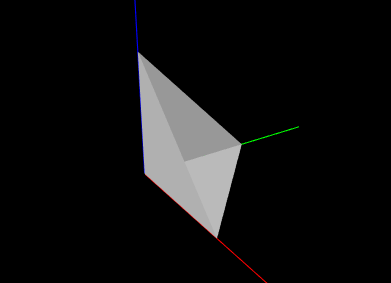
\includegraphics[]{images/drawOpenTet}
\else
 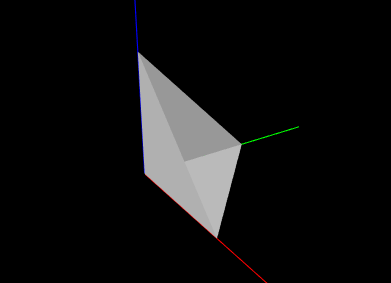
\includegraphics[width=3.75in]{images/drawOpenTet}
\fi
\end{center}
\caption{An open tetrahedron, with the viewer also displaying the world
frame x-y-z axes (as red, green and blue lines) to help show its
orientation.}
\label{drawOpenTet:fig}
\end{figure}
%

Another pair of methods are available for drawing solid triangles:
%
\begin{lstlisting}[]
void drawTriangle (Vector3d pnt0, Vector3d pnt1, Vector3d pnt2);
void drawTriangle (float[] pnt0, float[] pnt1, float[] pnt2);
\end{lstlisting}
%
Each of these draws a single triangle, with a normal computed
automatically with respect to the counter-clockwise orientation of the
vertices.

\begin{sideblock}
Note: as with drawing single points and lines, the single triangle
methods are inefficient. For rendering large numbers of triangles, one
should use either the {\it draw mode} methods of Section
\ref{drawMode:sec}, or the {\it render objects} described in Section
\ref{renderObjects:sec}.
\end{sideblock}

When drawing triangles, the renderer can be asked to
draw the {\it front} face, {\it back} face, or both faces. The
methods to control this are:
%
\begin{lstlisting}[]
FaceStyle getFaceStyle ();
void setFaceStyle (FaceStyle mode);
\end{lstlisting}
%
where \javaclassAlt{maspack.render.Renderer\$FaceStyle}{FaceStyle}
is an enumerated type of \javaclass[maspack.render]{Renderer}
with the possible values:

\begin{description}

\item[FRONT:]\mbox{} 

Draw the front face

\item[BACK:]\mbox{} 

Draw the back face

\item[FRONT\_AND\_BACK:]\mbox{} 

Draw both faces

\item[NONE:]\mbox{} 

Draw neither face

\end{description}
The example below draws a simple open tetrahedron with one face missing:
%
\begin{lstlisting}[]
import maspack.matrix.Vector3d;
import maspack.render.*;
import maspack.render.Renderer.FaceStyle;
...
   
   public void render (Renderer renderer, int flags) {
      // the corners of the tetrahedron
      Vector3d p0 = new Vector3d (0, 0, 0);
      Vector3d p1 = new Vector3d (1, 0, 0);
      Vector3d p2 = new Vector3d (0, 1, 0);
      Vector3d p3 = new Vector3d (0, 0, 1);
         
      // render both sides of each triangle:
      renderer.setFaceStyle (FaceStyle.FRONT_AND_BACK); 
      
      renderer.drawTriangle (p0, p2, p1);
      renderer.drawTriangle (p0, p3, p2);
      renderer.drawTriangle (p0, p1, p3);
      
      renderer.setFaceStyle (FaceStyle.FRONT); // restore default
   }
\end{lstlisting}
%
The result is drawn using the renderer's default gray color, as seen
in Figure \ref{drawOpenTet:fig}.

\subsection{Colors and associated attributes}
\label{colors:sec}

The renderer maintains a set of attributes for controlling the color,
reflectance and emission characteristics of whatever primitives or
shapes are currently being drawn. Color values are stored as RGBA
(red, green, blue, alpha) or RGB (red, green, blue) values in the
range $[0,1]$. The attributes closely follow the OpenGL model for
lighting materials and include:

\begin{description}

\item[Front color:]\mbox{} 

Specifies the reflected RGBA values for diffuse
and ambient lighting.  The default value is opaque gray: $(0.5, 0.5,
0.5, 1.0)$.

\item[Back color:]\mbox{} 

Optional attribute, which, if not {\tt null},
specifies the reflected RGBA values for diffuse and ambient lighting
for back faces only. Otherwise, the front color is used. The
default value is {\tt null}.

\item[Specular:]\mbox{} 

Specifies the reflected RGB values for specular lighting.
The default value is $(0.1, 0.1, 0.1)$.

\item[Emission:]\mbox{}

Specifies the RGB values for emitted light.  The
default value is $(0, 0, 0)$.

\item[Shininess:]\mbox{}

Specifies the specular exponent of the lighting
equation, in the range $[0, 128]$. The default value is 32.

\end{description}

The resulting appearance of subsequently rendered primitives or shapes
depends on the values of these attributes along with the shading
settings (Section \ref{shading:sec}). When lighting is disabled (by
calling {\tt setShading(Shading.NONE)}), then rendering is done in a
uniform color using only the {\it front color} (diffuse/ambient)
attribute.

The primary methods for setting the color attributes are:
%
\begin{lstlisting}[]
void setFrontColor (float[] rgba);
void setBackColor (float[] rgba);
void setSpecular (float[] rgb);
void setEmission (float[] rgb);
void setShininess (float s);
\end{lstlisting}
%
where {\tt rgba} and {\tt rgb} are arrays of length 4 or 3 that
provide the required RGBA or RGB values. The {\tt rgba} arguments may
also have a length of 3, in which case an alpha value of 1.0 is
assumed. For \javamethod[maspack.render.Renderer]{setBackColor()},
{\tt rgba} may also be {\tt null}, which will cause the back color to
be cleared.

Most commonly, there is no difference between the desired front and
back colors, in which case one can simply use the various {\tt
setColor} methods instead:
%
\begin{lstlisting}[]
void setColor (Color color);
void setColor (float[] rgba);
void setColor (float r, float g, float b);
void setColor (float r, float g, float b, float a);
void setFrontAlpha (float a);
\end{lstlisting}
%
These take RGB or RGBA values and set the front color, while at the
same time clearing the back color, so that the front color is
automatically applied to back faces. The method
\javamethod[maspack.render.Renderer]{setFrontAlpha()} independently
sets the alpha value for the front color.

To query the color attributes, one may use:
%
\begin{lstlisting}[]
float[] getFrontColor (float[] rgba);
float[] getBackColor (float[] rgba);
float[] getSpecular (float[] rgb);
float[] getEmission (float[] rgb);
float getShininess ();
\end{lstlisting}
%
The first four of these return the relevant RGBA or RGB values as an
array of floats. Applications may supply the float arrays using the
arguments {\tt rgba} or {\tt rgb}; otherwise, if these arguments are
{\tt null}, the necessary float arrays will be allocated. If no back
color is set, then
\javamethod[maspack.render.Renderer]{getBackColor()} will return {\tt
null}.

\subsubsection{Highlighting}
\label{highlighting:sec}

The renderer supports the notion of {\it highlighting}, which allows
the application to indicate to the renderer that subsequently rendered
components should be drawn in a highlighted manner. This is typically
used to show (visually) that they are {\it selected} in some way.

The highlighting style used by the renderer can be queried
using the method
%
\begin{lstlisting}[]
HighlightStyle getHighlightStyle();
\end{lstlisting}
%
At present, only two values of
\javaclassAlt{maspack.render.Renderer\$HighlightStyle}%
{HighlightStyle}
are supported:

\begin{description}

\item[COLOR:]\mbox{}

Highlighting is done by rendering with a distinct color.

\item[NONE:]\mbox{}

Highlighting is disabled.

\end{description}

The color used for color-based highlighting can be queried using
%
\begin{lstlisting}[]
void getHighlightColor (float[] rgb);
\end{lstlisting}
%

To enable or disable highlighting, the application can use
the methods 
%
\begin{lstlisting}[]
void setHighlighting (boolean enable)
boolean getHighlighting ()
\end{lstlisting}
%
\begin{figure}[t]
\begin{center}
\iflatexml
 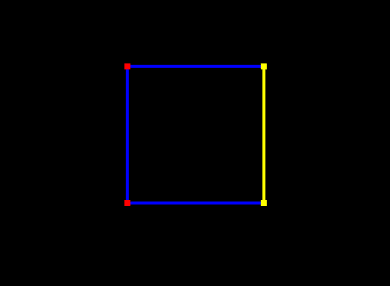
\includegraphics[]{images/selectedSquare}
\else
 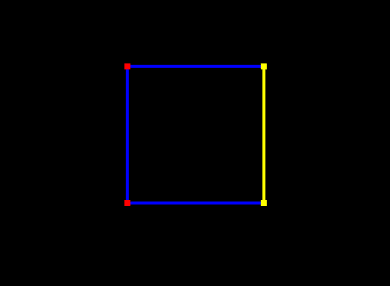
\includegraphics[width=3.75in]{images/selectedSquare}
\fi
\end{center}
\caption{Simple square with two points and one edge highlighted.}
\label{selectedSquare:fig}
\end{figure}
%
As an illustration, we alter the square drawing example of Section
\ref{singlePointsLines:sec} to highlight the corners corresponding
to points {\tt p1} and {\tt p1}, as well as the edge
between {\tt p1} and {\tt p1}:
%
\begin{lstlisting}[]
import java.awt.Color;
import maspack.matrix.Vector3d;
import maspack.render.*;
import maspack.render.Renderer.Shading;
...
   
   public void render (Renderer renderer, int flags) {
       // the corners of the square
      Vector3d p0 = new Vector3d (0, 0, 0);
      Vector3d p1 = new Vector3d (1, 0, 0);
      Vector3d p2 = new Vector3d (1, 0, 1);
      Vector3d p3 = new Vector3d (0, 0, 1);
      
      renderer.setShading (Shading.NONE); // turn off lighting
   
      renderer.setPointSize (6);
      renderer.setColor (Color.RED);
      renderer.drawPoint (p0);
      renderer.setHighlighting (true); // turn highlighting on
      renderer.drawPoint (p1);
      renderer.drawPoint (p2);
      renderer.setHighlighting (false); // turn highlighting off
      renderer.drawPoint (p3);
   
      renderer.setLineWidth (3);
      renderer.setColor (Color.BLUE);
      renderer.drawLine (p0, p1);
      renderer.setHighlighting (true); // turn highlighting on
      renderer.drawLine (p1, p2);
      renderer.setHighlighting (false); // turn highlighting off
      renderer.drawLine (p2, p3);        
      renderer.drawLine (p3, p0);        
   
      renderer.setShading (Shading.FLAT); // restore default shading
   }
\end{lstlisting}
%
The result, assuming a highlight style of
\javaclassAlt{maspack.render.Renderer\$HighlightStyle\#COLOR}%
{HighlightStyle.COLOR} and a yellow
highlight color, is shown in Figure \ref{selectedSquare:fig}.

\subsection{Drawing using draw mode}
\label{drawMode:sec}

For convenience, the renderer provides a {\it draw mode} in which
primitive sets consisting of points, lines and triangles can be assembled
by specifying a sequence of vertices and (if necessary) normals,
colors, and/or texture coordinates between calls to
\javamethodAlt{maspack.render.Renderer.beginDraw(DrawMode)}{beginDraw(mode)}
and \javamethod[maspack.render.Renderer]{endDraw()}. Because draw mode
allows vertex and normal information to be collected together and sent
to the GPU all at one time (when {\tt endDraw()} is called), it can be
significantly more efficient than the single point, line and triangle
methods described in the previous sections. (However, using {\it
render objects} can be even more efficient, as described in Section
\ref{renderObjects:sec}.)

\begin{table}[h]
\begin{center}
\begin{tabular}{|lll|}
\hline
DrawMode & Description & Equivalent OpenGL Mode\\
\hline
{\tt POINTS} & A set of independent points & {\tt GL\_POINTS} \\
{\tt LINES} & A set of line segments, with two vertices 
per segment & {\tt GL\_LINES}\\
{\tt LINE\_STRIP} & A line strip connecting the vertices in order &
{\tt GL\_LINE\_STRIP}\\
{\tt LINE\_LOOP} & A line loop connecting the vertices in order &
{\tt GL\_LINE\_LOOP}\\
{\tt TRIANGLES} & A set of triangles, with three vertices
per triangle & {\tt GL\_TRIANGLES}\\
{\tt TRIANGLES\_STRIP} & A triangle strip & {\tt GL\_TRIANGLE\_STRIP} \\
{\tt TRIANGLE\_FAN} & A triangle fan &
{\tt GL\_TRIANGLE\_FAN}\\
\hline
\end{tabular}
\end{center}
\caption{Draw mode primitive types.}
\label{DrawMode:tab}
\end{table}

Draw mode is closely analgous to {\it immediate mode} in older
OpenGL specifications. The types of primitive sets that may be formed from
the vertices are defined by
\javaclass[maspack.render]{Renderer\$DrawMode} and summarized in Table
\ref{DrawMode:tab}.
The primitive type is specified by the {\tt mode} argument of the
\javamethodAlt{maspack.render.Renderer.beginDraw(DrawMode)}{beginDraw(mode)}
call that initiates draw mode.

Between calls to {\tt beginDraw(mode)} and {\tt endDraw()}, vertices
may be added using the methods
%
\begin{lstlisting}[]
void addVertex (float px, float py, float pz);
void addVertex (double px, double py, double pz);
void addVertex (Vector3d pnt);
\end{lstlisting}
%
each of which creates and adds a single vertex for the specified
point.
Normals may be specified using
\begin{lstlisting}[]
void setNormal (float nx, float ny, float nz);
void setNormal (double nx, double ny, double nz);
void setNormal (Vector3d nrm);
\end{lstlisting}
%
It is not necessary to specify a normal for each vertex. Instead, the
first {\tt setNormal} call will specify the normal for all vertices
defined to that point, and all subsequent vertices until the next {\tt
setNormal} call. If no {\tt setNormal} call is made while in draw mode,
then the vertices will not be
associated with any normals, which typically means that the primitives
will be rendered as black unless lighting is disabled (Section
\ref{shading:sec}).

It is also possible to specify per-vertex colors during draw mode.
This can be done by calling any
of the methods of Section \ref{colors:sec} that cause the front color
to be set. The indicated front color will then be assigned to vertices
defined up to that point, and all subsequent vertices until the next
call that sets the front color. The primitives will then be rendered
using {\it vertex coloring}, in which the vertex color values are
interpolated to determine the color at any given point in a primitive.
This color overrides the current front (or back) color value (or mixes
with it; see Section \ref{colorMixing:sec}).  If vertex colors are not
specified, then the primitives will be rendered using the color
attributes that were in effect when draw mode was first entered.

Finally, per-vertex texture coordinates can be specified within draw
mode. The methods for doing this are analagous to those for setting
normals,
%
\begin{lstlisting}[]
void setTextureCoord (float tx, float ty);
void setTextureCoord (double tx, double ty);
void setTextureCoord (Vector2d tex);
\end{lstlisting}
%
where 
\javaclass[maspack.matrix]{Vector2d} is defined in {\tt maspack.matrix}.
Texture coordinates are required for any rendering that involves
texture mapping, including color, normal or bump maps (Section
\ref{mappings:sec}).

When draw mode is exited by calling {\tt endDraw()}, the specified
vertices, along with any normal, color or texture information, is sent
to the GPU and rendered as the specified primitive set, using the
current settings for shading, point size, line width, etc.

As an example, the code below uses draw mode to implement the square
drawing of Section \ref{singlePointsLines:sec} (which is shown in Figure
\ref{drawSquare:fig}):
%
\begin{lstlisting}[]
import java.awt.Color;
import maspack.matrix.Vector3d;
import maspack.render.*;
import maspack.render.Renderer.Shading;
import maspack.render.Renderer.DrawMode;
...
   
   public void renderDrawMode (Renderer renderer) {
      // the corners of the square
      Vector3d p0 = new Vector3d (0, 0, 0);
      Vector3d p1 = new Vector3d (1, 0, 0);
      Vector3d p2 = new Vector3d (1, 0, 1);
      Vector3d p3 = new Vector3d (0, 0, 1);
      
      renderer.setShading (Shading.NONE);  // turn off lighting
   
      renderer.setPointSize (6);
   
      renderer.beginDraw (DrawMode.POINTS);
      renderer.setColor (Color.RED);
      renderer.addVertex (p0);
      renderer.addVertex (p1);
      renderer.addVertex (p2);
      renderer.addVertex (p3);
      renderer.endDraw();
   
      renderer.setLineWidth (3);
      renderer.setColor (Color.BLUE);
      renderer.beginDraw (DrawMode.LINE_LOOP);
      renderer.addVertex (p0);
      renderer.addVertex (p1);
      renderer.addVertex (p2);
      renderer.addVertex (p3);
      renderer.endDraw();
   
      renderer.setShading (Shading.FLAT);  // restore lighting
   }
\end{lstlisting}
%
Note that no normals need to be specified since both primitive sets
are rendered with lighting disabled.

Another example uses draw mode to implement the partial tetrahedron
example from Section \ref{singleTriangles:sec} (which is shown in Figure
\ref{drawOpenTet:fig}):
%
\begin{lstlisting}[]
import maspack.matrix.Vector3d;
import maspack.render.*;
import maspack.render.Renderer.FaceStyle;
import maspack.render.Renderer.DrawMode;
...

   public void render (Renderer renderer, int flags) {
      // the corners of the tetrahedron
      Vector3d p0 = new Vector3d (0, 0, 0);
      Vector3d p1 = new Vector3d (1, 0, 0);
      Vector3d p2 = new Vector3d (0, 1, 0);
      Vector3d p3 = new Vector3d (0, 0, 1);
      
      // render both sides of each triangle:
      renderer.setFaceStyle (FaceStyle.FRONT_AND_BACK); 
   
      renderer.beginDraw (DrawMode.TRIANGLES);
      // first triangle
      renderer.setNormal (0, 0, -1); // normal along -z
      renderer.addVertex (p0); 
      renderer.addVertex (p2);
      renderer.addVertex (p1);
      // second triangle
      renderer.setNormal (-1, 0, 0); // normal along -x
      renderer.addVertex (p0); 
      renderer.addVertex (p3);
      renderer.addVertex (p2);
      // third triangle
      renderer.setNormal (0, -1, 0); // normal along -y
      renderer.addVertex (p0);
      renderer.addVertex (p1);
      renderer.addVertex (p3);
      renderer.endDraw();
   
      renderer.setFaceStyle (FaceStyle.FRONT); // restore default
   }
\end{lstlisting}
%
Note that because for this example we are displaying shaded faces, it
is necessary to specify a normal for each triangle.

%
\begin{figure}[t]
\begin{center}
\iflatexml
 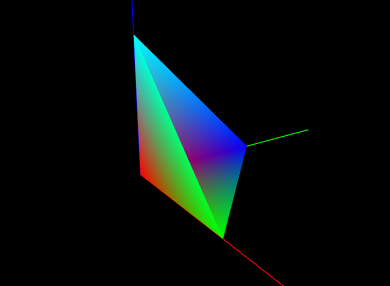
\includegraphics[]{images/coloredTet}
\else
 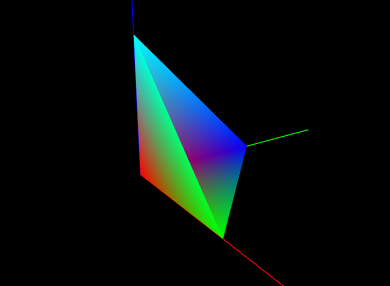
\includegraphics[width=3.75in]{images/coloredTet}
\fi
\end{center}
\caption{An open tetrahedron, drawn with colors specified at
each vertex, which causes the renderer to initiate {\it vertex coloring}
and interpolate the vertex colors across each face.}
\label{coloredTet:fig}
\end{figure}
%

As a final example, we show the tetrahedon example again, but this
time with colors specified for each vertex, which initiates {\it
vertex coloring}.  Vertices {\tt p0}, {\tt p1}, {\tt p2}, and {\tt p3}
are associated with the colors {\tt RED}, {\tt GREEN}, {\tt BLUE}, and
{\tt CYAN}, respectively. The corresponding code looks like this:
%
\begin{lstlisting}[]
   renderer.beginDraw (DrawMode.TRIANGLES);
   // first triangle
   renderer.setNormal (0, 0, -1);
   renderer.setColor (Color.RED);
   renderer.addVertex (p0); 
   renderer.setColor (Color.BLUE);
   renderer.addVertex (p2);
   renderer.setColor (Color.GREEN);
   renderer.addVertex (p1);
   // second triangle
   renderer.setNormal (-1, 0, 0);
   renderer.setColor (Color.RED);
   renderer.addVertex (p0); 
   renderer.setColor (Color.CYAN);
   renderer.addVertex (p3);
   renderer.setColor (Color.BLUE);
   renderer.addVertex (p2);
   // third triangle
   renderer.setNormal (0, -1, 0);
   renderer.setColor (Color.RED);
   renderer.addVertex (p0);
   renderer.setColor (Color.GREEN);
   renderer.addVertex (p1);
   renderer.setColor (Color.CYAN);
   renderer.addVertex (p3);
   renderer.endDraw();
\end{lstlisting}
%
and the rendered result is shown in Figure \ref{coloredTet:fig}.

\subsection{Drawing solid shapes}

For convenience, the renderer provides a number of methods for drawing
solid shapes. These include spheres, cylinders, cubes, boxes, arrows,
spindles, cones, and coordinate axes.

Methods for drawing spheres include
%
\begin{lstlisting}[]
void drawSphere (Vector3d pnt, double rad);
void drawSphere (float[] pnt, double rad);   
\end{lstlisting}
%
both of which draw a sphere with radius {\tt rad} centered at the
point {\tt pnt}, using the current color and shading settings.  For
drawing cylinders, arrows, or spindles, one can use
%
\begin{lstlisting}[]
void drawCylinder (float[] pnt0, float[] pnt1, double rad, boolean capped);
void drawArrow (float[] pnt0, float[] pnt1, double rad, boolean capped);
void drawSpindle (float[] pnt0, float[] pnt1, double rad);
\end{lstlisting}
%
each of which draws the indicated shape between points {\tt pnt0} and
{\tt pnt1} with a cylindrical radius of {\tt rad}, again using the
current color and shading. The argument {\tt capped} for cylinders and
arrows indicates whether or not a solid cap should be drawn over any
otherwise open ends. For arrows, the arrow head size is based on the
radius and line segment length.

A cone can be drawn similarly to a cylinder, using
%
\begin{lstlisting}[]
void drawCone (float[] pnt0, float[] pnt1, rad0, rad1, capped);
\end{lstlisting}
%
with the only difference being that there are now two radii, {\tt
rad0} and {\tt rad1}, at each end.

\begin{figure}[ht]
\begin{center}
   \begin{tabular}{ccc}
      \iflatexml
         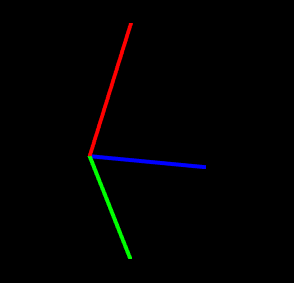
\includegraphics[]{images/coordAxes} &
         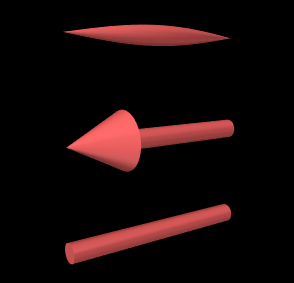
\includegraphics[]{images/solidLines} &
         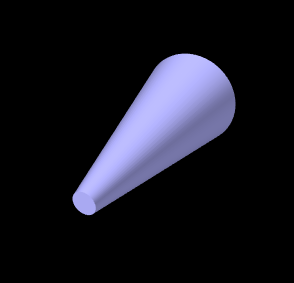
\includegraphics[]{images/solidCone}\\
      \else
         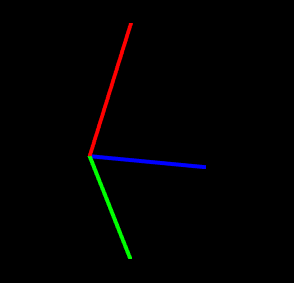
\includegraphics[width=2in]{images/coordAxes} &
         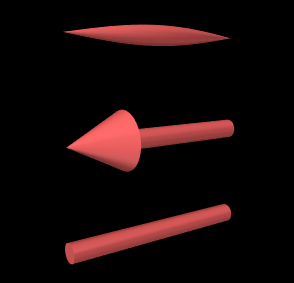
\includegraphics[width=2in]{images/solidLines} &
         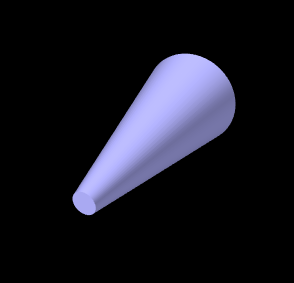
\includegraphics[width=2in]{images/solidCone}\\
      \fi
   \end{tabular}
\end{center}
\caption{Some of the solids that can be drawn by the renderer.  From
left to right: coordinate axes; spindle, arrow, and cylinder (capped);
a cone.}
\label{solids:fig}
\end{figure}

To draw cubes and boxes, one may use
%
\begin{lstlisting}[]
void drawCube (Vector3d pnt, double width);
void drawCube (float[] pnt, double width);
void drawBox (Vector3d pnt, Vector3d widths);
void drawBox (float[] pnt, double wx, double wy, double wz);
void drawBox (RigidTransform3d TBM, Vector3d widths);
\end{lstlisting}
%
The {\tt drawCube} methods draw an axis-aligned cube with a specified
{\tt width} centered on the point {\tt pnt}. Similarly, the first two
{\tt drawBox} methods draw an axis-aligned box with the indicated x,
y, and z widths. Finally, the last {\tt drawBox} method draws a box
centered on, and aligned with, the coordinate frame defined (with
respect to model coordinates) by the 
\javaclass[maspack.matrix]{RigidTransform3d} {\tt TBM}.

When rendering the curved solids described above, the renderer must
create surface meshes that approximate their shapes. The resolution
used for doing this can be controlled using a parameter called the
{\it surface resolution}. This is defined to be the number of line
segments that would be used to approximate a circle, and this level of
resolution is then employed to create the mesh. The renderer
initializes this parameter to a reasonable default value, but
applications can query or modify it as needed using the following
methods:
%
\begin{lstlisting}[]
int getSurfaceResolution();
void setSurfaceResolution (int nsegs);
\end{lstlisting}
%

Coordinate axes can be drawn to show the position and orientation of a
spatial coordinate frame:
%
\begin{lstlisting}[]
void drawAxes (RigidTransform3d T, double len, width, boolean highlight);
void drawAxes (RigidTransform3d T, double[] lens, width, boolean highlight);
\end{lstlisting}
%
For these, the coordinate frame is described (with respect to the current
model coordinates) by a 
\javaclass[maspack.matrix]{RigidTransform3d} {\tt T}. The first method
draws the frame's axes
as lines with the specified length {\tt len} and {\tt
width}. The second method allows different lengths ({\tt lens}) to be
specified for each axis. The axis lines are rendered using regular
pixel-based lines with non-shaded colors, with the $x$, $y$, and $z$
axes normally being colored {\tt red}, {\tt green}, and {\tt blue}.
However, if {\tt highlight} is {\tt true} and the highlight
style is 
\javaclassAlt{maspack.render.Renderer\$HighlightStyle\#COLOR}%
{HighlightStyle.COLOR}
(Section \ref{highlighting:sec}), then all axes are drawn
using the using the highlight color.

Some of the solids are illustrated in Figure \ref{solids:fig}.

\subsection{Shading and color mixing}
\label{shading:sec}

Shading determines the coloring of each rendering primitive (point,
line or triangle), as seen from the eye, as a result of its color
attributes, surface normals and the current lighting conditions. At
any given point on a primitive, the {\it rendered color} is the
coloring seen from the eye that results from the incident
illumination, color attributes, and surface normal at that point. In
general, the rendered color varies across the primitive.  How this
variation is handled depends on the {\it shading}, defined by
\javaclass[maspack.render]{Renderer\$Shading}:

%
\begin{description}

\item[FLAT:]\mbox{}

The rendered color is determined at the first vertex and applied to the
entire primitive. This makes it easy to see the individual primitives,
which can be desirable under some circumstances. Only one normal needs
to be specified per primitive.

\item[SMOOTH:]\mbox{}

Rendered colors are computed across the primitive, based on
interpolated normal information, resulting in a smooth appearance. The
interpolation technique depends on the renderer.  OpenGL 2
implementations use Gouraud shading, while the OpenGL 3 renderer uses
Phong shading.

\item[METAL:]\mbox{}

Rendered colors are computed using a smooth shading technique that may
be more appropriate to metalic objects. For some renderer
implementations, there may be no difference between {\tt METAL} and
{\tt SMOOTH}.

\item[NONE:]\mbox{}

Lighting is disabled. The rendered color becomes the diffuse color,
which is applied uniformly across the primitive. No normals need to be
specified.

\end{description}
%

\begin{figure}[ht]
\begin{center}
   \begin{tabular}{ccc}
      \iflatexml
         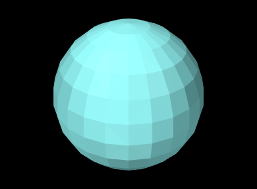
\includegraphics[]{images/sphereFlatShading} &
         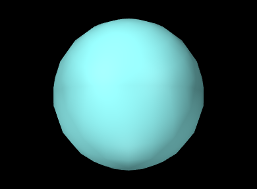
\includegraphics[]{images/sphereSmoothShading} &
         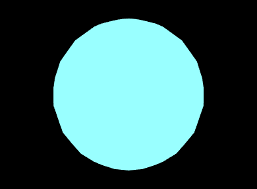
\includegraphics[]{images/sphereNoShading}\\
      \else
         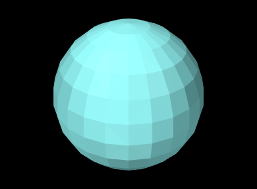
\includegraphics[width=2in]{images/sphereFlatShading} &
         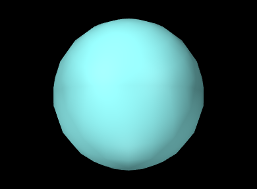
\includegraphics[width=2in]{images/sphereSmoothShading} &
         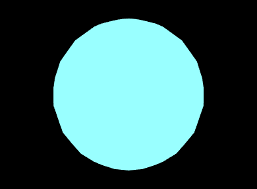
\includegraphics[width=2in]{images/sphereNoShading}\\
      \fi
   \end{tabular}
\end{center}
\caption{A polygonal sphere with shading set to {\tt FLAT} (left),
{\tt SMOOTH} (middle), and {\tt NONE} (right).}
\label{shading:fig}
\end{figure}

Figure \ref{shading:fig} shows different shading methods applied
to a sphere.

The shading can be controlled and queried using the
following methods,
%
\begin{lstlisting}[]
Shading getShading();
Shading setShading (Shading shading);
\end{lstlisting}
%
where \javamethod[maspack.render.Renderer]{setShading()} returns the
previous shading setting.

Lighting is often disabled, using {\tt Shading.NONE}, when rendering
pixel-based points and lines. That's because normal information is not
naturally defined for these primitives, and also because even if
normal information were to be provided, shading could make them either
invisible or hard to see from certain viewing angles.

\subsection{Vertex coloring, and color mixing and interpolation}
\label{colorMixing:sec}

As mentioned in Section \ref{drawMode:sec}, it is possible to specify
{\it vertex coloring} for a primtive, in which vertex color values are
interpolated to determine the color at any given point in the
primitive. Vertex colors can be specified by calling {\tt setColor}
primitives while in draw mode. They can also be specified as part of a
{\tt RenderObject} (Section \ref{renderObjects:sec}).

When vertex coloring is used, the interpolated vertex colors either
replace or are combined with the current front (or back) diffuse color
at each point in the primitive. Other color attributes, such as
emission and specular, are unchanged. If lighting is disabled, then
the rendered color is simply set to the resulting vertex/diffuse color
combination.

Whether the vertex color replaces or combines with the underlying
diffuse color is controlled by the enumerated type
\javaclass[maspack.render]{Renderer\$ColorMixing}, which has four
different values:
%
\begin{center}
\begin{tabular}{|ll|}
\hline 
REPLACE & replace the diffuse color (default behavior) \\
MODULATE & multiplicatively combine with the diffuse color\\
DECAL & combine with the diffuse color based on the latter's alpha value \\
NONE & diffuse color is unchanged (vertex colors are ignored)\\
\hline
\end{tabular}
\end{center}
%

\begin{figure}[ht]
\begin{center}
   \begin{tabular}{ccc}
      \iflatexml
         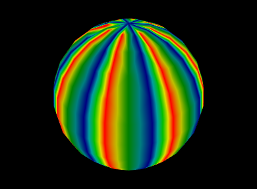
\includegraphics[]{images/coloredVerticesUnshaded} &
         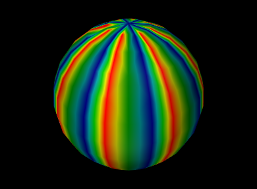
\includegraphics[]{images/coloredVerticesShaded} &
         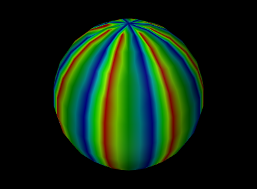
\includegraphics[]{images/coloredVerticesModulated}\\
      \else
         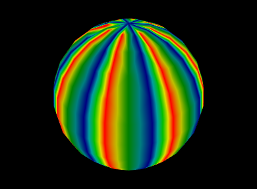
\includegraphics[width=2in]{images/coloredVerticesUnshaded} &
         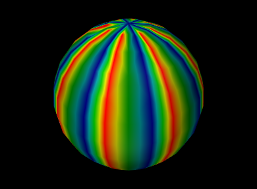
\includegraphics[width=2in]{images/coloredVerticesShaded} &
         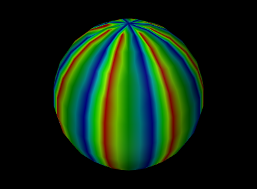
\includegraphics[width=2in]{images/coloredVerticesModulated}\\
      \fi
   \end{tabular}
\end{center}
\caption{Vertex coloring applied to the pale blue sphere of Figure
\ref{shading:sec}.  Left: shading={\tt NONE}, color mixing={\tt
REPLACE}; Middle: shading={\tt SMOOTH}, color mixing={\tt REPLACE};
Right: shading={\tt SMOOTH}, color mixing={\tt MODULATE}. The right
sphere is slightly darker because {\tt MODULATE} causes the vertex
coloring to be multiplied by the underlying blue color, reducing its
intensity.}
\label{vertexColoring:fig}
\end{figure}

Color mixing can be controlled using these methods:
%
\begin{lstlisting}[]
ColorMixing getVertexColorMixing();
void setVertexColorMixing (ColorMixing cmix); 
boolean hasVertexColorMixing (ColorMixing cmix);
\end{lstlisting}
%
A given Renderer implementation may not support all color mixing
modes, and so the
\javamethod[maspack.render.Renderer]{hasVertexColorMixing()} can be
used to query if a given mixing mode is supported.  The OpenGL 2
renderer implementation does not support {\tt MODULATE} or {\tt
DECAL}. Some examples of vertex coloring with different shading
and color mixing settings
are shown in Figure \ref{vertexColoring:fig}.

\begin{sideblock}
The renderer's default color mixing mode is {\tt MODULATE}. This has
the advantage of allowing rendered objects to still appear differently
when highlighting is enabled and the highlight style is
\javaclassAlt{maspack.render.Renderer\$HighlightStyle\#COLOR}%
{HighlightStyle.COLOR} (Section \ref{highlighting:sec}), since the
highlight color is combined with the vertex color rather than being
replaced by it.
\end{sideblock}

%\begin{sideblock}
%OpenGL 2 renderer implementations have another limitation in that
%vertex coloring will not interpolate properly unless the current
%shading is set to {\tt SMOOTH} or {\tt METAL}. Otherwise, instead of
%interpolating the vertex colors, the primitive will simply be colored
%entirely using the color specified for the primitive's first vertex.
%\end{sideblock}

\begin{figure}[ht]
\begin{center}
   \begin{tabular}{cc}
      \iflatexml
         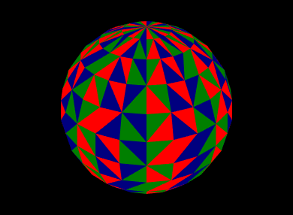
\includegraphics[]{images/coloredFacesUnshaded} &
         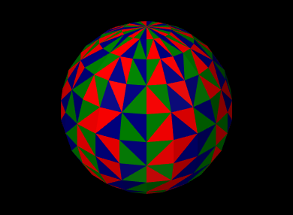
\includegraphics[]{images/coloredFacesShaded}\\
      \else
         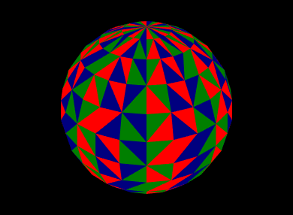
\includegraphics[width=2.5in]{images/coloredFacesUnshaded} &
         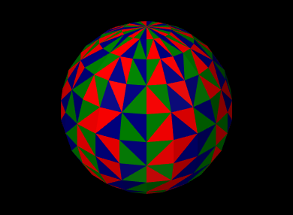
\includegraphics[width=2.5in]{images/coloredFacesShaded}\\
      \fi
   \end{tabular}
\end{center}
\caption{Vertex coloring applied to a sphere, only with the vertices
for each face now being given the same colors so as to color each face
uniformly.  Left: shading={\tt NONE}, color mixing={\tt REPLACE};
Right: shading={\tt SMOOTH}, color mixing={\tt REPLACE}.}
\label{faceColoring:fig}
\end{figure}

Vertex coloring can be used in different ways. Assigning different
colors to the vertices of a primitive will result in a blending of
those colors within the primitive (Figures \ref{coloredTet:fig} and
\ref{vertexColoring:fig}). Assigning the {\it same} colors to the
vertices of a primitive can be used to give each primitive a uniform
color. Figure \ref{faceColoring:fig} shows vertex coloring applied to
the same sphere as Figures \ref{shading:sec} and
\ref{vertexColoring:fig}, only with the vertices for each face
being uniformly set to red, green or blue, resulting in
uniformly colored faces.

\begin{figure}[ht]
\begin{center}
   \begin{tabular}{cc}
      \iflatexml
         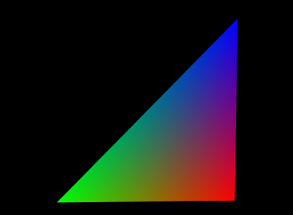
\includegraphics[]{images/RGBinterpolation} &
         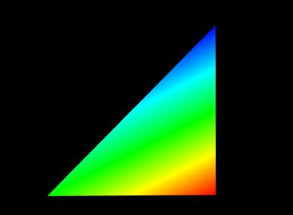
\includegraphics[]{images/HSVinterpolation}\\
      \else
         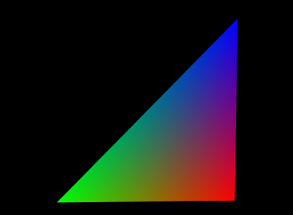
\includegraphics[width=2.5in]{images/RGBinterpolation} &
         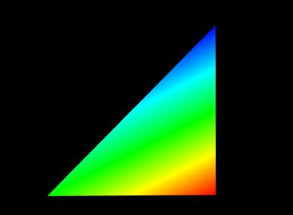
\includegraphics[width=2.5in]{images/HSVinterpolation}\\
      \fi
   \end{tabular}
\end{center}
\caption{RGB interpolation (left) and HSV interpolation (right),
applied to a triangle with vertices colored red,
green and blue.}
\label{RGBvsHSV:fig}
\end{figure}

When using vertex coloring, the interpolation of colors across the
primitive can be done either in RBG or HSV space. HSV stands for hue,
saturation, and value (or brightness), and it is often the best
interpolation method to use when the vertex colors have a uniform
brightness that the interpolation should preserve. This leads to a
``rainbow'' look that is common in situations like color-based stress
plots. Figure \ref{RGBvsHSV:fig} illustrates the difference between
RGB and HSV interpolation.

Color interpolation is specified with the enumerated type
\javaclass[maspack.render]{Renderer\$ColorInterpolation}, which
currently has the two values {\tt RGB} and {\tt HSV}. Within the
renderer, it can be controlled using the methods
%
\begin{lstlisting}[]
ColorInterpolation getColorInterpolation();
void setColorInterpolation (ColorInterpolation interp);
\end{lstlisting}
%

\subsection{Changing the model matrix}
\label{modelMatrix:sec}

When point positions are specified to the renderer, either as the
arguments to various draw methods, or for specifying vertex
locations in draw mode, the positions are assumed to be defined with
respect to the current {\it model} coordinate frame. As described in
Section \ref{coordinateFrames:sec}, this is one of the three primary
coordinate frames associated with the viewer, with the other two
being the {\it world} and {\it eye} frames.

The relationship between model and world frames is controlled by the
{\it model matrix} $\X_{MW}$, which is a $4 \times 4$ homogeneous
affine transform that transforms points in model coordinates (denoted
by ${}^M\p$) to world coordinates (denoted by ${}^W\p$), according to
%
\begin{equation*}
\matl {}^W\p \\ 1 \matr \;=\;
\X_{MW} \matl {}^M\p \\ 1 \matr.
\end{equation*}
%
Initially the world and model frames are coincident, so that $\X_{MW}
= \I$. Rendering methods often redefine the model matrix, allowing
object geometry to be specified in a conveniently defined local
coordinate frame, and, more critically, allowing the predefined
geometry associated with existing rendering objects (Section
\ref{renderObjects:sec}) or built-in drawing methods to be used at
different scales and poses throughout the scene.  Methods for querying
and controlling the model matrix include:
%
\begin{lstlisting}[]
AffineTransform3dBase getModelMatrix();
void getModelMatrix (AffineTransform3d XMW);

void setModelMatrix (AffineTransform3dBase XMW);
void mulModelMatrix (AffineTransform3dBase X);
void translateModelMatrix (double tx, double ty, double tz);
void rotateModelMatrix (double zdeg, double ydeg, double xdeg);
void scaleModelMatrix (double s);

void pushModelMatrix();
boolean popModelMatrix();
\end{lstlisting}
%
Both \javamethod[maspack.render.Renderer]{getModelMatrix()} and
\javamethodAlt{maspack.render.Renderer.getModelMatrix(AffineTransform3d)}%
{getModelMatrix(XMW)} return the current model matrix value (where the
value returned by the first method should not be modified).
\javaclass[maspack.matrix]{AffineTransform3dBase} is a base class defined
in {\tt maspack.matrix} and represents a $4 \times 4$ homogeneous transform
that is either a rigid transform
(of type
\javaclass[maspack.matrix]{RigidTransform3d}) or an affine transform
(of type \javaclass[maspack.matrix]{AffineTransform3d}).
\javamethodAlt{maspack.render.Renderer.setModelMatrix()}{setModelMatrix(XMW)}
explicitly sets the model matrix, while
\javamethodAlt{maspack.render.Renderer.setModelMatrix()}{mulModelMatrix(X)}
post-multiplies the current matrix by another rigid or
affine transform $\X$, which is equivalent to
setting
%
\begin{equation*}
\X_{MW} := \X_{MW} \, \X.
\end{equation*}
%
\javamethodAlt{maspack.render.Renderer.translateModelMatrix()}%
{translateModelMatrix(tx,ty,tz)} and
\javamethodAlt{maspack.render.Renderer.rotateModelMatrix()}%
{rotateModelMatrix(zdeg,ydeg,xdeg)} translate or rotate the model
frame by post-multiplying the model matrix by a rigid transform
describing either a translation ({\tt tx}, {\tt ty}, {\tt tz}), or
a rotation formed by three successive rotations: {\tt zdeg} degrees
about the $z$ axis, {\tt ydeg} degrees about the new $y$ axis, and
finally {\tt xdeg} degrees about the new $x$ axis.
\javamethodAlt{maspack.render.Renderer.scaleModelMatrix()}{scaleModelMatrix(s)}
scales the current model frame by
post multiplying the model matrix by a uniform scaling transform
%
\begin{equation*}
\X \equiv \matl
s & 0 & 0 & 0 \\
0 & s & 0 & 0 \\
0 & 0 & s & 0 \\
0 & 0 & 0 & 1 \\
\matr.
\end{equation*}
%
Finally, \javamethod[maspack.render.Renderer]{pushModelMatrix()} and
\javamethod[maspack.render.Renderer]{popModelMatrix()} save and
restore the model matrix from an internal stack. It is common to
wrap changes to the model matrix inside calls to {\tt
pushModelMatrix()} and {\tt popModelMatrix()} so that the model matrix
is preserved unchanged for subsequent use elsewhere:
%
\begin{lstlisting}[]
renderer.pushModelMatrix();
   ...
   renderer.mulModelMatrix(X);
   ... specific rendering code ...
   ...
renderer.popModelMatrix();
\end{lstlisting}
%

\subsection{Render properties and RenderProps}
\label{RenderProps:sec}

The {\tt maspack.render} package defines an object called
\javaclass[maspack.render]{RenderProps} which encapsulates many of the
properties that are needed to describe how an oject should be
rendered. These properties control the color, size, and style of the
three primary rendering primitives: faces, lines, and points, and all
are exposed using the {\tt maspack.properties}
package, so that they can be easily set from a GUI or inherited from
ancestor components.

A renderable object can maintain its own {\tt RenderProps} object, and
use the associated properties as it wishes to control rendering from
within its {\tt render()} method. Objects maintaining their own {\tt
RenderProps} can declare this by implementing the
\javaclass[maspack.render]{HasRenderProps} interface, which
declares the methods
%
\begin{lstlisting}[]
  setRenderProps (RenderProps props); // set render properties
  RenderProps getRenderProps();       // get render properties (read-only)
  RenderProps createRenderProps();    // create render properties for this object
\end{lstlisting}
%
\begin{sideblock}
It is not intended for {\tt RenderProps} to encapsulate {\it all}
properties relevant to the rendering of objects, but only those which
are commonly encountered. Any particular renderable may still need to
define and maintain more specialized rendering properties.
\end{sideblock}

\begin{sideblock}
Renderable objects that implement both
\javaclass[maspack.render]{HasRenderProps} and
\javaclass[maspack.render]{IsSelectable} (an extension of
\javaclass[maspack.render]{IsRenderable} for selectable objects
described in Section \ref{objectSelection:sec}) are identified by the
combined interface \javaclass[maspack.render]{Renderable}.
\end{sideblock}

\subsubsection{Drawing points and lines as 3D solid objects}

{\tt RenderProps} contains two properties, {\sf pointStyle} and {\sf
lineStyle}, that indicate whether points and lines should be drawn
using standard pixel-based primitives or some type of solid 3D
geometry.  Often, the latter can be preferable for visualization and
graphical selection.  {\sf pointStyle} and {\sf lineStyle} are
described by the enumerated types
\javaclass[maspack.render]{Renderer\$PointStyle} and
\javaclass[maspack.render]{Renderer\$LineStyle}, respectively, which
contain the following entries:

\begin{center}
\begin{tabular}{|ll|}
\hline 
{\it PointStyle:} & \\
\hline 
POINT & pixel-based point \\
SPHERE & solid sphere \\
CUBE & solid cube\\
\hline
{\it LineStyle:} & \\
\hline 
LINE & pixel-based line \\
CYLINDER & solid cylinder \\
SOLID\_ARROW & solid arrow \\
SPINDLE & spindle (an ellipsoid tapered at each end) \\
\hline
\end{tabular}
\end{center}

The size (in pixels) for pixel-based points is controlled by the
property {\sf pointSize}, whereas the radius for spherical points and
half-width for cubic points is controlled by {\sf pointRadius}.
Likewise, the width (in pixels) for pixel-based lines is controlled by
{\sf lineWidth}, whereas the radii for lines rendered as cylinders,
arrows or spindles is controlled by {\sf lineRadius}.

\subsubsection{RenderProps taxonomy}

All of the {\tt RenderProps} properties are listed in table 
\ref{RenderProps:tab}.
Values for the {\sf shading}, {\sf
faceStyle}, {\sf lineStyle} and {\sf pointStyle} properties are
defined using the following enumerated types:
\javaclass[maspack.render]{Renderer\$Shading}, 
\javaclass[maspack.render]{Renderer\$Faces}, 
\javaclass[maspack.render]{Renderer\$PointStyle}, 
and 
\javaclass[maspack.render]{Renderer\$LineStyle}.
Colors are specified using {\tt java.awt.Color}.

\begin{table}[h]
\begin{center}
\begin{tabular}{|lll|}
\hline property & purpose & default value \\ \hline
%Generic properties:
visible & whether or not the component is visible & {\tt true} \\
alpha & transparency for diffuse colors (range 0 to 1) & 1 (opaque) \\
lighting & lighting style:
({\tt FLAT}, {\tt SMOOTH}, {\tt METAL}, {\tt NONE}) & {\tt FLAT}\\
shininess & shininess parameter (range 0 to 128) & 32 \\
specular & specular color components & {\tt null} \\
%Face related properties &
\hline
faceStyle &
which polygonal faces are drawn ({\tt FRONT}, {\tt BACK},
{\tt FRONT\_AND\_BACK}, {\tt NONE}) & {\tt FRONT} \\
faceColor &
diffuse color for drawing faces & {\tt GRAY} \\
backColor &
diffuse color used for the backs of faces.
If {\tt null}, {\tt faceColor} is used. & {\tt null} \\
drawEdges & hint that polygon edges should be drawn explicitly & {\tt false} \\
\hline
colorMap & 
color map properties (see Section \ref{mappings:sec})& {\tt null}\\
normalMap & 
normal map properties (see Section \ref{mappings:sec})& {\tt null}\\
bumpMap & 
bump map properties (see Section \ref{mappings:sec})& {\tt null}\\
% Edge related properties &
\hline
edgeColor & diffuse color for edges & {\tt null} \\
edgeWidth & edge width in pixels & 1 \\
% Line related properties &
\hline
lineStyle: &
how lines are drawn ({\tt CYLINDER}, {\tt LINE}, or {\tt SPINDLE}) & 
{\tt LINE} \\
lineColor & diffuse color for lines & {\tt GRAY} \\
lineWidth & width in pixels when {\tt LINE} style is selected & 1 \\
lineRadius & radius when {\tt CYLINDER} or {\tt SPINDLE} style is selected &
1 \\
% Point related properties &
\hline
pointStyle & how points are drawn ({\tt SPHERE} or {\tt POINT}) & {\tt POINT} \\
pointColor & diffuse color for points & {\tt GRAY} \\
pointSize & point size in pixels when {\tt POINT} style is selected & 1 \\
pointRadius & sphere radius when {\tt SPHERE} style is selected & 1 \\
\hline
\end{tabular}
\end{center}
\caption{Render properties and their default values.}
\label{RenderProps:tab}
\end{table}

In addition to colors for points, lines, and faces, there are also
optional colors for edges and back faces. Edge colors (and edge
widths) are provided in case an object has both lines and faces, and
may want to render the edges of the faces in a color separate from the
line color, particularly if {\sf drawEdges} is set to {\tt
true}. ({\tt PolygonalMeshRenderer}, described in Section
\ref{meshRendering:sec}, responds to {\sf drawEdges} by drawing the
polygonal edges using {\sf edgeColor}.)  Back face colors are provided
so that back faces can be rendered using a different color than the
front face.

Exactly how a component interprets its render properties is up to the
component (and more specifically, up to the {\tt render()} method for that
component).  Not all render properties are relevant to all components,
particularly if the rendering does not use all of the rendering
primitives. For example, some components may use only
the point primitives and others may use only
the line primitives. For this reason, some components use subclasses
of {\tt RenderProps}, such as
\javaclass[maspack.render]{PointRenderProps} and
\javaclass[maspack.render]{LineRenderProps}, that expose only a subset
of the available render properties. All renderable components provide
the method
\javamethod[maspack.render.HasRenderProps]{createRenderProps()} that
will create and return a {\tt RenderProps} object suitable for that
component.

\subsubsection{Renderer methods that use RenderProps}

{\tt Renderer} provides a number of convenience methods for setting
attributes and drawing primitives and shapes based on information
supplied by {\tt RenderProps}.

For drawing points and lines, there are
%
\begin{lstlisting}[]
void drawPoint (RenderProps props, float[] pnt, boolean highlight);

void drawLine (
   RenderProps props, float[] pnt0, float[] pnt1, boolean highlight);

void drawLine (
   RenderProps props, float[] pnt0, float[] pnt1, float[] color, 
   boolean capped, boolean highlight);
\end{lstlisting}
%
{\tt drawPoint()} draws a point at location {\tt pnt} using the {\sf
pointStyle}, {\sf pointColor}, {\sf pointSize}, {\sf pointRadius} and
{\sf shading} properties of {\tt props}, while the {\tt drawLine}
methods draw a line between {\tt pnt0} and {\tt pnt1} using the {\sf
lineStyle}, {\sf lineColor}, {\sf lineSize}, {\sf lineRadius} and {\sf
shading} properties. The second {\tt drawLine} method also allows an
alternate {\tt color} to be specified, as well as whether or not the
line shape should be {\tt capped} (if appropriate).  Another method,
%
\begin{lstlisting}[]
void drawArrow (
   RenderProps props, float[] pnt0, float[] pnt1, float[] color, 
   boolean capped, boolean highlight);
\end{lstlisting}
%
is identical to the second {\tt drawLine} method above except that the line
style {\tt LineStyle.SOLID\_ARROW} is assumed. For all methods, the
{\tt highlight} argument can be used to request that the primitive
or shape be
drawn with highlighting enabled (Section
\ref{highlighting:sec}).

To draw a line strip, one can use
%
\begin{lstlisting}[]
void drawLineStrip (
   RenderProps props, Iterable<float[]> pnts, LineStyle style, boolean highlight);
\end{lstlisting}
%
which draws a line strip with the specified {\tt pnts}, using the
indicated {\tt style} along with the {\sf lineColor}, {\sf lineSize},
{\sf lineRadius} and {\sf shading} properties of {\tt props}. The
strip is rendered with highlighting if {\tt highlight} is {\tt true}.

There are also methods for setting the color attributes associated
with {\sf pointColor}, {\sf lineColor}, {\sf edgeColor}, or
{\sf faceColor}:
%
\begin{lstlisting}[]
void setPointColoring (RenderProps props, boolean highlight);
void setLineColoring (RenderProps props, boolean highlight);
void setEdgeColoring (RenderProps props, boolean highlight);
void setFaceColoring (RenderProps props, boolean highlight);
void setFaceColoring (RenderProps props, float[] rgba, boolean highlight);
\end{lstlisting}
%
These set the renderer's front color attribute to the value of the
indicated color property, use {\tt props} to also set the shininess
and specular attributes, and restore emission to its default renderer
value. The first three methods clear the back color attribute, while
the {\tt setFace} methods set it to the {\sf backColor} value of {\tt
props}. {\tt setEdgeColoring()} uses {\sf lineColor} if {\sf
edgeColor} is {\tt null}, and the second {\tt setFace} method allows
an alternate front color to be supplied as {\tt rgba}. For all
methods, highlighting is enabled or disabled based on the value of
{\tt highlight}.  A related method is
%
\begin{lstlisting}[]
void setPropsColoring (RenderProps props, float[] rgba, boolean highlight);
\end{lstlisting}
%
which behaves similarly except that the color is explicitly specified
using {\tt rgba}.

Lastly, there are methods to set the shading:
%
\begin{lstlisting}[]
Shading setPropsShading (RenderProps props);
Shading setPointShading (RenderProps props);
Shading setLineShading (RenderProps props);
\end{lstlisting}
%
{\tt setPointShading()} sets the shading to the {\sf shading} property
of {\tt props} and returns the previous value.  {\tt
setPointShading()} does the same, unless {\sf pointStyle} is {\tt
PointStyle.POINT}, in which case lighting is turned off by setting the
shading to {\tt Shading.NONE}.  Similarly, {\tt setLineShading()}
turns off the lighting if {\sf lineStyle} is {\tt LineStyle.LINE}.

\subsection{Screen information and 2D rendering}

The {\it screen} refers to the 2 dimensional pixelized display on
which the viewer ultimately renders the scene. There is a direct
linear mapping between the view plane (Figure
\ref{coordinateFrames:sec}) and the screen.

While the renderer does not give the application control over the
screen dimensions, it does allow them to be queried using
%
\begin{lstlisting}[]
int getScreenHeight();
int getScreenWidth();
\end{lstlisting}
%
It also allows distances in pixel space to be converted to
distances in world space via
%
\begin{lstlisting}[]
double distancePerPixel (Vector3d p);
double centerDistancePerPixel ();
\end{lstlisting}
%
\javamethodAlt{maspack.render.Renderer.distancePerPixel()}%
{distancePerPixel(p)} computes the displacement distance of a point
{\tt p}, in a plane parallel to the view plane, that corresponds to a
screen displacement of one pixel.
\javamethod[maspack.render.Renderer]{centerDistancePerPixel()}
computes the same thing with {\tt p} given by the center point
(Section \ref{coordinateFrames:sec}).

A renderer may also support {\it 2D mode} to facilitate the rendering
of 2D objects directly in screen coordinates. 2D mode
can be queried with the following methods:
%
\begin{lstlisting}[]
boolean has2DRendering();            // true if renderer supports 2D mode
boolean is2DRendering();             // true if renderer is in 2D mode
\end{lstlisting}
%
In order for an object to be rendered in 2D, the renderable should
return the flag
\javaclassAlt{maspack.render.IsRenderable\#TWO\_DIMENSIONAL}%
{IsRenderable.TWO\_DIMENSIONAL} from its
\javamethod[maspack.render.IsRenderable]{getRenderHints()} method.
The viewer will then call the {\tt render()} method in two dimensional
mode, with the view matrix set to the identity, and the projection and
model matrices set to provide an orthographic view (Figure
\ref{orthographic:fig}) with the world frame located at the lower left
screen corner, the $x$ axis horizontal and pointing to the right, and
the $y$ axis vertical. The top right corner of the screen corresponds
to the point $(w, h)$, where $w$ and $h$ are the width and height of
screen returned by 
\javamethod[maspack.render.Renderer]{getScreenWidth()} and
\javamethod[maspack.render.Renderer]{getScreenHeight()}.
Lighting is also disabled and the depth buffer
is turned off, so that rendered objects will always be visible in the
order they are drawn. 

If a different scaling or origin for the x-y plane is desired,
the application can call the renderer method
%
\begin{lstlisting}[]
void setModelMatrix2d (double left, double right, double top, double bottom)
\end{lstlisting}
%
which will reset the model matrix so that the lower left and upper right
of the screen correspond to the points
{\tt (left, bottom)} and {\tt (right, top)}, respectively.

\begin{figure}[t]
\begin{center}
\iflatexml
 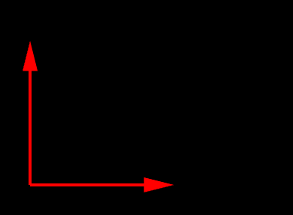
\includegraphics[]{images/arrowFrame}
\else
 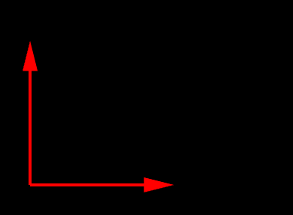
\includegraphics[width=3.25in]{images/arrowFrame}
\fi
\end{center}
\caption{Simple coordinate axes drawn using 2D mode.}
\label{arrowFrame:fig}
\end{figure}
%

The following example shows the code for a renderable that uses 2D
rendering to draw a pair of coordinate axes in the lower left screen
corner, with the result shown in Figure \ref{arrowFrame:fig}.  Its
{\tt getRenderHints()} method returns the {\tt TWO\_DIMENSIONAL} flag
to ensure that {\tt render()} is called in 2D mode.  The axis
arrowheads are drawn using the method {\tt drawArrowHead}, which draws
an arrowhead in a fixed location and orientation, in combination with
changes to the model matrix (Section \ref{coordinateFrames:sec}) to
adjust the base location and orientation as required.
%
\begin{lstlisting}[]
import java.awt.Color;
import maspack.matrix.Vector3d;
import maspack.render.*;
import maspack.render.Renderer.DrawMode;
...

   // ensure that render() is called in 2d mode
   int getRenderHints() {
      return TWO_DIMENSIONAL;
   }
   
   // draw a 2D arrowhead with a given size, centered on the origin
   private void drawArrowHead (Renderer renderer, int size) {
      Vector3d p0 = new Vector3d(size, 0, 0);
      Vector3d p1 = new Vector3d(-size, size/2, 0);
      Vector3d p2 = new Vector3d(-size, -size/2, 0);
      renderer.drawTriangle (p0, p1, p2);
   }         
   
   public void render (Renderer renderer, int flags) {
   
      // draw simple 2d coordinate frame axes in 2D mode
   
      int margin = 40;                   // distance from screen edge
      int arrowSize = 20;                // size of the axis arrows
      double length = 
         0.6*renderer.getScreenHeight(); // axis length
   
      // po, px and py are the origin and the x and y axis end points
      Vector3d po = new Vector3d (margin, margin, 0);
      Vector3d px = new Vector3d (margin+length, margin, 0);
      Vector3d py = new Vector3d (margin, margin+length, 0);
   
      renderer.setColor (Color.RED);
      
      // draw the axis lines with a line strip
      renderer.setLineWidth (4);
      renderer.beginDraw (DrawMode.LINE_STRIP);
      renderer.addVertex (px);
      renderer.addVertex (po);
      renderer.addVertex (py);
      renderer.endDraw();
      renderer.setLineWidth (1);
   
      // then draw an arrowhead at the tip of the x and y axes
      renderer.translateModelMatrix (px.x, px.y, 0);
      drawArrowHead (renderer, arrowSize);
      renderer.translateModelMatrix (py.x-px.x, py.y-px.y, 0);
      renderer.rotateModelMatrix (90, 0, 0);
      drawArrowHead (renderer, arrowSize);
   }
\end{lstlisting}
%

\subsection{Depth offsets}
\label{depthOffset:sec}

Sometimes, when drawing different primitives that lie on the same
plane, the depth buffer cannot properly resolve which primitive should
be visible. This artifact is known as ``z fighting''. The renderer
provides a means to address it via the method
%
\begin{lstlisting}[]
void setDepthOffset (double zoffset)
\end{lstlisting}
%
This modifies the projection matrix to incorporate a small offset (in
clip coordinates) along the eye frame's $z$ axis, so that subsequently
rendered components are rendered slightly closer to (or farther from)
the eye. Each unit of offset equals one unit of depth buffer
precision. The depth offset can be queried using
\javamethod[maspack.render.Renderer]{getDepthOffset()}, and the
default value is 0.

\begin{figure}[ht]
\begin{center}
   \begin{tabular}{cc}
      \iflatexml
         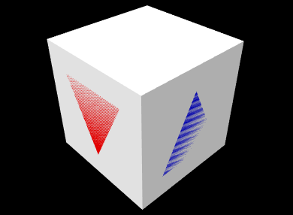
\includegraphics[]{images/trianglesOnCube} &
         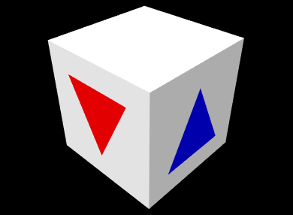
\includegraphics[]{images/trianglesOnCubeOffset}\\
      \else
         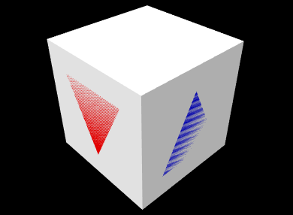
\includegraphics[width=2.5in]{images/trianglesOnCube} &
         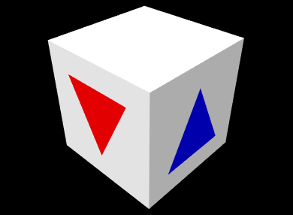
\includegraphics[width=2.5in]{images/trianglesOnCubeOffset}\\
      \fi
   \end{tabular}
\end{center}
\caption{Triangles drawn on the surface of a cube. This nominally
results in z fighting (left), which can be removed
by setting a depth offset (right).}
\label{depthExample:fig}
\end{figure}

The listing below shows an example in which two colored triangles are
drawn on faces of a cube. If no depth offset is set, the triangles
compete for visibility with the underlying cube faces (Figure
\ref{depthExample:fig}, left). To resolve this, the {\tt render()}
method sets a depth offset to move the triangles slighting closer to
the eye.
%
\begin{lstlisting}[]
import java.awt.Color;
import maspack.matrix.Vector3d;
import maspack.render.*;
...

   public void render (Renderer renderer, int flags) {
   
      // draw the cube
      renderer.setColor (Color.WHITE);
      renderer.drawCube (Vector3d.ZERO, 2.0);
   
      // points for the triangles on the cube faces
      Vector3d p0 = new Vector3d (   0, -1.0, -0.6);
      Vector3d p1 = new Vector3d ( 0.6, -1.0,  0.6);
      Vector3d p2 = new Vector3d (-0.6, -1.0,  0.6);
   
      Vector3d p3 = new Vector3d ( 1.0, -0.6, -0.6);
      Vector3d p4 = new Vector3d ( 1.0,  0.6, -0.6);
      Vector3d p5 = new Vector3d ( 1.0,    0,  0.6);
   
      // set a depth offset so the triangles will be visible ...
      renderer.setDepthOffset (1);
   
      // ... and draw the triangles
      renderer.setColor (Color.RED);
      renderer.drawTriangle (p0, p1, p2);
      renderer.setColor (Color.BLUE);
      renderer.drawTriangle (p3, p4, p5);
   }
\end{lstlisting}
%
\begin{sideblock}
z-fighting may still occur if the plane in which the fighting occurs
is tilted significantly with respect to the eye.  In some situations
it may be desirable to mitigate this with a larger offset value.
\end{sideblock}

\subsection{Maintaining the graphics state}

%
\begin{table}[h]
\begin{center}
\begin{tabular}{|llll|}
\hline
Attribute & Description & Default value & Restored\\
\hline
front color & diffuse/ambient color & (0.5, 0.5, 0.5, 1.0) & no\\
back color & optional color for back faces & {\tt null} & yes\\
emission & emission color & (0, 0, 0) & yes\\
specular & specular color & (0.1, 0.1, 0.1) & yes\\
shininess & specular color & 32 & yes\\
\hline
color interpolation & interpolation method for vertex colors & {\tt RGB}& yes\\
face style & whether to draw front or back faces & {\tt FRONT}& yes\\
line width & width of pixel-based lines & 1& yes\\
point size & size of pixel-based points & 1& yes\\
\hline
model matrix & transform from model to world coordinates & IDENTITY& yes\\
highlighting & highlight drawn primitives & {\tt false}& yes\\
shading & primitive shading based on normal information & {\tt FLAT}& yes\\
surface resolution & internal curved surface resolution & 32& yes\\
vertex color mixing & how to combine underlying and vertex colors &
{\tt REPLACE}& yes\\
depth offset & moves rendered objects slightly along the eye z axis & 0 & yes\\
\hline        
color map & color map properties (Section \ref{mappings:sec}) & {\tt null}& yes\\
normal map & normal map properties (Section \ref{mappings:sec}) & 
{\tt null}& yes\\
bump map & bump map properties (Section \ref{mappings:sec}) & {\tt null}& yes\\
\hline
\end{tabular}
\end{center}
\caption{Attributes comprising the renderer graphics state, with their 
default values and whether or not they are restored by the renderer.}
\label{graphicsState:tab}
\end{table}
%

Attributes such as colors, face styles, line widths, matrix values,
etc., constitute the {\it graphics state} associated with the
renderer.  Table \ref{graphicsState:tab} summarizes these attributes
and their default values. The last column, {\it Restored}, indicates
if the renderer will restore the attribute to its default value after
calling each renderable's {\tt render()} method in the repaint step.
At present, only the front color is not restored. All other
attributes will therefore be set to their default value at the
beginning of any {\tt render()} method {\it when} that method is being
called by the renderer.

Note that in some cases, a renderable's {\tt render()} method may {\it
not} be called by the render. This will occur, for instance, when a
renderable takes direct control of rendering its subcomponents, and
calls their {\tt render()} methods directly. In such cases, it will be
up to either the subcomponents or the parent to maintain the graphics
state as required. There are several ways to acccomplish this.

One way is to save and restore each attribute that is modified.  To
facilitate this, most attribute {\tt set} methods return the
attribute's previous value.  Save and restore can then be done using
blocks of the form
%
\begin{lstlisting}[]
   Shading savedShading = renderer.setShading (Shading.METAL);

   ... rendering operations ...

   renderer.setShading (savedShading);
\end{lstlisting}
%
As mentioned earlier, the model matrix can be saved and restored
using the following:
%
\begin{lstlisting}[]
   renderer.pushModelMatrix();
   renderer.setModelMatrix(TMW);
   
   ... rendering operations ...

   renderer.popModelMatrix();
\end{lstlisting}
%
Alternatively, if it is sufficient to restore an attribute to its
default value, one can do that directly:
%
\begin{lstlisting}[]
   renderer.setShading (Shading.METAL);

   ... rendering operations ...

   renderer.setShading (Shading.FLAT);
\end{lstlisting}
%
Finally, the renderer method
\javamethod[maspack.render.Renderer]{restoreDefaultState()} can be
used to restore that default state of all attributes except the
front color:
%
\begin{lstlisting}[]
   ... rendering operations ...
 
   renderer.restoreDefaultState (/*strictChecking=*/true);
\end{lstlisting}
%
If {\tt true}, the {\tt strictChecking} argument causes an exception
to be thrown if the renderer is still in a draw mode block (Section
\ref{drawMode:sec}) or the model matrix stack is not empty.  {\tt
restoreDefaultState()} is used internally by the renderer to restore
state.

\subsection{Text rendering}

Some renderer implementations provide the ability to render text
objects, using fonts described by the Java class {\tt java.awt.Font}. 
Support for text rendering can be querired using the
method \javamethod[maspack.render.Renderer]{hasTextRendering()}.
The methods for drawing text include:
%
\begin{lstlisting}[]
double drawText (String str, float[] pos, double emSize);
double drawText (Font font, String str, float[] pos, double emSize);
double drawText (String str, Vector3d pos, double emSize);
double drawText (Font font, String str, float[] pos, double emSize);
\end{lstlisting}
%
Each of these draws the string {\tt str} in the x-y plane in model
coordinates, using either a specified font or a default. The starting
position of the lower left corner of the text box is given by {\tt
pos}, and {\tt emSize} gives the size of an ``em'' unit. The methods
return the horizontal advance distance of the draw operation.

Other supporting methods for text rendering include:
%
\begin{lstlisting}[]
void setDefaultFont(Font font);
Font getDefaultFont();
Rectangle2D getTextBounds(Font font, String str, double emSize);
\end{lstlisting}
%
These set and query the default font, and return the bounds of a text
box in a {\tt java.awt.geom.Rectangle2D}.

\begin{figure}[ht]
\begin{center}
   \iflatexml
      \includegraphics[]{images/drawText}
   \else
      \includegraphics[width=3.75in]{images/drawText}
   \fi
\end{center}
\caption{Text rendering example.}
\label{drawText:fig}
\end{figure}

Listing \ref{drawText:lst} below shows the code for the text rendering
shown in Figure \ref{drawText:fig}.
%
\begin{lstlisting}[caption={Using the renderer to draw text.},
label=drawText:lst]
import java.awt.Font;
import java.awt.Font;
import java.awt.GraphicsEnvironment;
import java.awt.geom.Rectangle2D;

import maspack.matrix.*;
import maspack.render.*;
...

   Font myComic;
   Font mySerif;

   void setupFonts() {
      GraphicsEnvironment env =
         GraphicsEnvironment.getLocalGraphicsEnvironment();
      for (Font font : env.getAllFonts ()) {
         if (font.getName().equals ("Comic Sans MS")) {
            myComic = font;
            break;
         }
      }
      if (myComic == null) {
         myComic = new Font(Font.MONOSPACED, Font.BOLD, 32);
      }
      else {
         myComic = myComic.deriveFont (Font.BOLD, 32);
      }
      mySerif = new Font(Font.SERIF, Font.PLAIN, 64);
   }

   public void render (Renderer renderer, int flags) {

      Vector3d pos = new Vector3d(-0.6, 0, 0);

      // draw text at (0,0)
      renderer.setColor (Color.WHITE);
      renderer.drawText ("Hello World!", pos, 0.2);

      // draw text rotated about the z axis
      renderer.setColor (Color.CYAN);
      String text = "Cowabunga";
      renderer.pushModelMatrix();
      renderer.rotateModelMatrix (30, 0, 0);
      pos.set (-0.3, 0.6, 0);
      renderer.drawText (myComic, "Cowabunga", pos, 0.25);
      renderer.popModelMatrix();

      // draw several centered lines, in a plane rotated about the x axis
      renderer.setColor (Color.ORANGE);
      renderer.pushModelMatrix();
      String[] textLines = new String[] {
         "Four score and", "seven years ago,",
         "in a galaxy", "far far", "away" };
      renderer.mulModelMatrix (
         new RigidTransform3d (0, -0.1, -1.0, 0, 0, -Math.toRadians(60)));
      pos.set (0, 0, 0);
      for (String line : textLines) {
         Rectangle2D rect = renderer.getTextBounds (mySerif, line, 0.25);
         pos.y -= rect.getHeight();
         pos.x = -rect.getWidth()/2;
         renderer.drawText (mySerif, line, pos, 0.25);
      }
      renderer.popModelMatrix();
   }
\end{lstlisting}
The method {\tt setupFonts()} is called outside the render method to
set up some fonts and store them in the member variables {\tt myComic}
and {\tt mySerif}.  Note that setting up fonts in general may be
system specific.  Three different blocks of text are then drawn within
the {\tt render()} method, with different colors, positions and
orientations. The last block consists of multiple lines, with
\javamethod[maspack.render.Renderer]{getTextBounds()} used to obtain
the text bounds necessary to center each line.

\section{Render Objects}
\label{renderObjects:sec}

In modern graphics interfaces, applications send geometric, color,
and texture information to the GPU, which then applies the various
computations associated with the graphics pipeline. Transferring this
data to the GPU can be an expensive activity, and efficient applications
try to minimize it. Modern OpenGL, in particular, requires
applications to bundle the geometric, color, and texture information
into buffer objects, which are transmitted to the GPU and then cached
there.  This generally increases efficiency because (a) large amounts
of data can be transferred at once, and (b) the cached data can be
reused in subsequent rendering operations.

For OpenGL renderer implementations, a buffer object must be created
and transmitted to the GPU once for every invocation of a {\tt draw}
method or {\tt beginDraw()/endDraw()} block. As a more efficient
alternative, applications can create instances of {\it render
objects}, which store geometric, color, and texture information and
manage the transmission of this data to the GPU. Essentially, a render
object provides a convenience wrapper for OpenGL-type buffer objects.
However, the use of render objects is generic and not limited to
OpenGL implementations of the renderer.

Render objects are implemented using the
\javaclass[maspack.render]{RenderObject} class, which
contains:

\begin{itemize}

\item {\it Attribute data}, including {\it positions}, and
(optionally) {\it normals}, {\it colors}, and {\it texture
coordinates}.

\item {\it vertex data}, where each vertex points to a single
position, as well as (optionally) a single normal, color, and texture
attribute.

\item {\it primitive data}, consisting of zero or more ``groups'' of
{\it points}, {\it lines}, and {\it triangles}.

\end{itemize}

%
\begin{figure}[t]
\begin{center}
\iflatexml
 \includegraphics[]{images/renderObject}
\else
 \includegraphics[width=4.5in]{images/renderObject}
\fi
\end{center}
\caption{Render object structure, showing the relationship between
attributes, vertices, and primitives.}
\label{renderObject:fig}
\end{figure}
%

To summarize, primitives are made of vertices, which are in turn
comprised of references to attributes (Figure \ref{renderObject:fig}).

Render objects can be created anywhere within the application program,
although care must be taken to synchronize their modification with the
{\tt render()} methods. While an easy way to do this is to create them
directly within the render method, care should then be taken to allow
them to persist between render invocations, since each time a new
object is created, all of its data must be transferred to the GPU. It
is recommended to create render objects within {\tt prerender()},
since this should automatically provide synchronization with both {\tt
render()} and any other thread this is modifying render data.  A
render object can itself be used to cache rendering data associated
with a dynamically varying object, in which case creating (or
updating) it from within the prerender method is even more
appropriate.

\subsection{Building a render object}
\label{buildingRenderObjects:sec}

Attributes can be added using a variety of
\javaclass[maspack.render]{RenderObject} methods, including:
%
\begin{lstlisting}[]
int addPosition (float px, float py, float pz);
int addPosition (Vector3d pos);
int addPosition (float[] pos);    // set by reference

int addNormal (float nx, float ny, float nz);
int addNormal (Vector3d nrm);
int addNormal (float[] nrm);      // set by reference

int addColor (float r, float g, float b, float a);
int addColor (Color color);
int addColor (byte[] rgba);       // set by reference

int addTextureCoord (float tx, float ty);
int addTextureCoord (Vector2d xy);
int addTextureCoord (float[] xy); // set by reference
\end{lstlisting}
%
Each of these creates an instance of the specified attribute, sets it
to the indicated value, adds it to the render object, and assigns it a
unique index, which is returned by the {\tt add} method. The index can
be referred to later when adding vertices, or when later changing the
attribute's value (Section \ref{modifyingObjects:sec}). Indices are
increased sequentially, starting from zero.

\begin{sideblock}
Methods above marked {\it ``set by reference''} use the supplied array to
directly store values within the attribute, so that subsequent changes to
the array's values will also cause the attribute's values to change.
\end{sideblock}

A vertex is defined by a 4-tuple of indices that can be used to refer
to a previously defined instance of each of the four attributes:
position, normal, color, and texture coordinate. A vertex does not
need to reference all attributes, but it is required that {\bf
all vertices have a consistent set of attributes} (e.g.~either all
vertices have a normal reference, or none do).  When adding a vertex, a
negative index indicates that the attribute is not present. Since a
vertex can refer to at most one of each attribute, this means that
when building primitives, it may be necessary to define multiple
vertices for the same position if different values are required for
the other attributes (e.g., normals, colors, or texture coordinates).
For example, for the corner of the cube at location $(-1,-1,-1)$,
there must be three vertices defined, one each with normals
$(-1,0,0)$, $(0,-1,0)$, and $(0,0,-1)$.

Referencing attributes by index allows for attributes to be reused,
and also for the numbers of any given attribute to vary. For example,
when rendering the faces of a solid cube, we typically need 24
vertices (4 for each of the 6 faces), but only 8 positions (one per
corner) and 6 normals (one per face). 

Vertices can be added using the 
\javaclass[maspack.render]{RenderObject} method
%
\begin{lstlisting}[]
int addVertex (int pidx, int nidx, int cidx, int tidx);
\end{lstlisting}
%
where {\tt pidx}, {\tt nidx}, {\tt cidx}, and {\tt tidx} are the
indices of the desired postion, normal, color and texture coordinate
attributes (or -1 for attributes that are undefined). The method
returns a unique index for the vertex, which can be referred to later
when adding primitives. Indices are increased sequentially, starting
from zero. 

Once vertices are created, they can be used to define and add
primitives. Three types of primitives are available: points (one
vertex each), lines (two vertices each), and triangles (three vertices
each). Methods for adding these include
%
\begin{lstlisting}[]
addPoint (int v0idx);
addLine (int v0idx, int v1idx);
addTriangle (int v0idx, int v1idx, int v2idx);
\end{lstlisting}
%
Each of these takes a set of vertex indices, creates the corresponding
primitive, and adds it to the current group for the that primitive
(primitive groups are discussed in Section \ref{primitiveGroups:sec}).

Once all the primitives have been added, 
the {\tt Renderer}
method \javamethod[maspack.render.Renderer]{draw(RenderObject)} can
then be used to draw all the primitives in the object using the
current graphics state. A variety of other {\tt draw} methods are
available for drawing subsets of primitives; these are detailed in
Section \ref{drawingRenderObjs:sec}.

There are no methods to remove individual attributes, vertices, or
primitives. However, as described in Section
\ref{modifyingObjects:sec}, it is possible to use
\javamethod[maspack.render.RenderObject]{clearAll()} to clear the
entire object, after which it may be rebuilt, or
\javamethod[maspack.render.RenderObject]{clearPrimitives()} to clear
just the primitive sets.

Listing \ref{renderObjTet:lst} gives a complete example combining the
above operations to create a render object that draws the open
tetrahedron described in Section \ref{singleTriangles:sec} and Figure
\ref{drawOpenTet:fig}. In this example, the object itself is created
using the method {\tt createTetRenderObject()}. This is in turn called
once within {\tt prerender()} to create the object and store it in the
member field {\tt myRob}, allowing it to then be used as needed within
{\tt render()}. As indicated above, it is generally recommended to
create or update render objects within the prerender method,
particularly if they need to be modfied to reflect dynamically
changing geometry or colors.
%
\begin{lstlisting}[caption={Construction and use of a render object to draw
a partial tetrahedron.}, 
label=renderObjTet:lst]
import maspack.render.*;
import maspack.render.Renderer.FaceStyle;
...

   RenderObject myRob;
   
   private RenderObject createTetRenderObject() {
      // the corners of the tetrahedron
      
      RenderObject robj = new RenderObject();
   
      // add positions and normals
      int pi0 = robj.addPosition (0, 0, 0);
      int pi1 = robj.addPosition (1, 0, 0);
      int pi2 = robj.addPosition (0, 1, 0);
      int pi3 = robj.addPosition (0, 0, 1);
   
      int ni0 = robj.addNormal (0, 0, -1);
      int ni1 = robj.addNormal (-1, 0, 0);
      int ni2 = robj.addNormal (0, -1, 0);
   
      // add three vertices per triangle, each with position and normal
      // information and color and texture coords undefined, and then
      // use these to define a triangle primitive
   
      int v0, v1, v2;
   
      // first triangle
      v0 = robj.addVertex (pi0, ni0, -1, -1);
      v1 = robj.addVertex (pi2, ni0, -1, -1);
      v2 = robj.addVertex (pi1, ni0, -1, -1);
      robj.addTriangle (v0, v1, v2);
   
      // second triangle
      v0 = robj.addVertex (pi0, ni1, -1, -1);
      v1 = robj.addVertex (pi3, ni1, -1, -1);
      v2 = robj.addVertex (pi2, ni1, -1, -1);
      robj.addTriangle (v0, v1, v2);
   
      // third triangle
      v0 = robj.addVertex (pi0, ni2, -1, -1);
      v1 = robj.addVertex (pi1, ni2, -1, -1);
      v2 = robj.addVertex (pi3, ni2, -1, -1);
      robj.addTriangle (v0, v1, v2);
   
      return robj;
   }
   
   public void prerender (RenderList list) {
      if (myRob == null) {
         myRob = createTetRenderObject();
      }
   }
         
   public void render (Renderer renderer, int flags) {
   
      renderer.setFaceStyle (FaceStyle.FRONT_AND_BACK); 
      renderer.draw (myRob);  // draw the render object
      renderer.setFaceStyle (FaceStyle.FRONT); 
   }
\end{lstlisting}

\subsection{``Current'' attributes}

Keeping track of attribute indices as described in Section
\ref{buildingRenderObjects:sec} can be tedious. Instead of doing this,
one can use the fact that every attribute {\tt add} method records the
index of the added attribute, which then denotes the ``current'' value
for that attribute.  The following methods can then be used to add a
vertex using various current attribute values:
%
\begin{lstlisting}[]
// use current position, normal, color and texture coords:
int addVertex ();              

// use position pidx with current normal, color and texture coords:
int addVertex (int pidx);

// use position pidx and normal nidx with current color and texture coords:
int addVertex (int pidx, int nidx);
\end{lstlisting}
If any of the attributes have no ``current'' value, then the
corresponding index value is -1 and that attribute will be undefined
for the vertex.

If desired, it is possible to set or query the current attribute
index, using methods of the form
%
\begin{lstlisting}[]
void setCurrent<Attribute>(int idx);
int getCurrent<Attribute>();
\end{lstlisting}
%
where {\tt <Attribute>} is {\tt Position}, {\tt Normal}, {\tt Color},
or {\tt TextureCoord} and {\tt idx} is the index of a currently added
attribute.
%
For convenience, another set of methods,
%
\begin{lstlisting}[]
int vertex (float px, float py, float pz);
int vertex (Vector3d pos);
\end{lstlisting}
%
will create a new position at the specified location, and then also create
a vertex using that position along with the current normal, color and
texture coords.

We now give some examples. First, Listing
\ref{renderObjTetCurrent:lst} changes the tetrahedron code in
Listing \ref{renderObjTet:lst} to use a current normal in
conjuction with
\javamethodAlt{maspack.render.RenderObject.vertex(float,float,float)}%
{vertex(px, py, pz)}.
%
\begin{lstlisting}[caption={Constructing a render object using current normals.},
label=renderObjTetCurrent:lst]
   // add three vertices per triangle, each with position and normal
   // information and color and texture coords undefined, and then
   // use these to define a triangle primitive

   int v0, v1, v2;

   // first triangle
   robj.addNormal (0, 0, -1);
   v0 = robj.vertex (0, 0, 0);
   v1 = robj.vertex (0, 1, 0);
   v2 = robj.vertex (1, 0, 0);
   robj.addTriangle (v0, v1, v2);

   // second triangle
   robj.addNormal (-1, 0, 0);
   v0 = robj.vertex (0, 0, 0);
   v1 = robj.vertex (0, 0, 1);
   v2 = robj.vertex (0, 1, 0);
   robj.addTriangle (v0, v1, v2);

   // third triangle
   robj.addNormal (0, -1, 0);
   v0 = robj.vertex (0, 0, 0);
   v1 = robj.vertex (1, 0, 0);
   v2 = robj.vertex (0, 0, 1);
   robj.addTriangle (v0, v1, v2);
\end{lstlisting}
%
One issue with using {\tt vertex(px, py, pz)} is that it creates a new
position for every vertex, even in situations where vertices can be
shared. The example above (implicitly) creates 9 positions where only
4 would be sufficient. Instead, one can create the positions
separately (as in Listing \ref{renderObjTet:lst}), and then use
\javamethodAlt{maspack.render.RenderObject.addVertex(int)}%
{vertex(pidx)} to add vertices created from predefined positions along
with current attribute values. Listing \ref{renderObjNormalsColors:lst}
does this for the tetrahedron, while also using a current color
to give each face it's own color. The rendered results are
shown in Figure \ref{coloredRenderObjTet:fig}.
%
\begin{figure}[t]
\begin{center}
\iflatexml
 \includegraphics[]{images/coloredRenderObjTet}
\else
 \includegraphics[width=3.75in]{images/coloredRenderObjTet}
\fi
\end{center}
\caption{An open tetrahedron drawn using a render object constructed
using a different current color for each face.}
\label{coloredRenderObjTet:fig}
\end{figure}
%
\begin{lstlisting}[caption={Constructing a render object using current normals
and colors.},label=renderObjNormalsColors:lst]
   // add positions and normals
   int pi0 = robj.addPosition (0, 0, 0);
   int pi1 = robj.addPosition (1, 0, 0);
   int pi2 = robj.addPosition (0, 1, 0);
   int pi3 = robj.addPosition (0, 0, 1);

   // add three vertices per triangle, each with position and normal
   // information and color and texture coords undefined, and then
   // use these to define a triangle primitive

   int v0, v1, v2;

   // first triangle
   robj.addNormal (0, 0, -1);
   robj.addColor (Color.CYAN);
   v0 = robj.addVertex (pi0);
   v1 = robj.addVertex (pi2);
   v2 = robj.addVertex (pi1);
   robj.addTriangle (v0, v1, v2);

   // second triangle
   robj.addNormal (-1, 0, 0);
   robj.addColor (Color.WHITE);
   v0 = robj.addVertex (pi0);
   v1 = robj.addVertex (pi3);
   v2 = robj.addVertex (pi2);
   robj.addTriangle (v0, v1, v2);

   // third triangle
   robj.addNormal (0, -1, 0);
   robj.addColor (Color.MAGENTA);
   v0 = robj.addVertex (pi0);
   v1 = robj.addVertex (pi1);
   v2 = robj.addVertex (pi3);
   robj.addTriangle (v0, v1, v2);
\end{lstlisting}

\subsection{Maintaining consistent attributes}

As mentioned earlier, all vertices within a render object must have a
consistent set of attributes. That means that if some vertices are
defined with normals or colors, they {\it all} must be defined with
normals or colors, even if it means giving some vertices ``dummy''
versions of these attributes for primitives that don't need them.

%
\begin{figure}[ht]
\begin{center}
\iflatexml
 \includegraphics[]{images/borderedTriangle}
\else
 \includegraphics[width=3.25in]{images/borderedTriangle}
\fi
\end{center}
\caption{A triangle with a separate red border.}
\label{borderedTriangle:fig}
\end{figure}
%

For example, suppose we wish to create an oject that draws a
triangular face surrounding by an outer border (Figure
\ref{borderedTriangle:fig}). One might write the following code to
create and draw the render object:
%
\begin{lstlisting}[]
import java.awt.Color;
import maspack.render.*;
import maspack.render.Renderer.Shading;
...

   RenderObject createRenderObj () {
                  
      RenderObject robj = new RenderObject();
      
      // add vertices for outer border - created without a normal
      robj.vertex (-0.8f, -0.5f, 0);
      robj.vertex ( 0.8f, -0.5f, 0);
      robj.vertex ( 0.0f,  1.0f, 0);
   
      // add points for triangle - create with a normal
      robj.addNormal (0, 0, 1f);
      robj.vertex (-0.64f, -0.4f, 0);
      robj.vertex ( 0.64f, -0.4f, 0);
      robj.vertex ( 0.0f,   0.8f, 0);
   
      // add outer border using first three vertices
      robj.addLine (0, 1);
      robj.addLine (1, 2);
      robj.addLine (2, 0);
   
      // add triangle using next three vertices
      robj.addTriangle (3, 4, 5);
   
      return robj;         
   }
   
   RenderObject myRob;
   
   public void render (Renderer renderer, int flags) {
      if (myRob == null) {
         myRob = createRenderObj ();
      }
      // draw border
      renderer.setShading (Shading.NONE); // turn off lighting
      renderer.setColor (Color.RED);
      renderer.setLineWidth (3);
      renderer.drawLines (myRob);
   
      // draw triangle
      renderer.setShading (Shading.FLAT); // reset shading
      renderer.setColor (Color.GRAY);
      renderer.drawTriangles (myRob);
   }
\end{lstlisting}
%
This creates a render object containing vertices for the border and
triangle, along with the line and triangle primitives. Then {\tt
render()} first draws the border and the triangle, using the
renderer's
\javamethodAlt{maspack.render.Renderer.drawLines(RenderObject)}%
{drawLines()} and
\javamethodAlt{maspack.render.Renderer.drawTriangles(RenderObject)}%
{drawTriangles()} methods (described in Section
\ref{drawingRenderObjs:sec}).  Because the border is drawn with
lighting disabled, no normal is required and so its vertices are
created without one. However, as written, this example will crash,
because the triangle vertices {\it do} contain a normal, and therefore
the border vertices must as well. The example can be fixed by moving
the {\tt addNormal()} call in front of the creation of the first three
vertices, which will then contain a normal even though it will remain
unused.

\subsection{Adding primitives in ``build'' mode}

The \javaclass[maspack.render]{RenderObject} can also be
systematically constructed using a ``build mode'', similar to the draw
mode described in Section \ref{drawMode:sec}.  Build mode can be
invoked for any of the primitive types defined by
\javaclassAlt{maspack.render.Renderer\$DrawMode}{DrawMode}
(Table \ref{DrawMode:tab}).

Primitive construction begins with
\javamethod[maspack.render.RenderObject]{beginBuild(DrawMode)} and
ends with \javamethod[maspack.render.RenderObject]{endBuild()}. While
in build mode, the application adds vertices using any of the methods
described in the previous sections. Then, when {\tt endBuild()} is
called, the render object uses those those vertices to create the
primitives that were specified by the {\tt mode} argument of {\tt
beginBuild(mode)}.

Listing \ref{renderObjCylinder:lst} shows a complete example where
build mode is used to create a {\tt RenderObject} for a cylinder.  In
this example, we first reserve memory for the required attributes,
vertices and triangles.  This is not a required step, but does help
with internal storage.  Then, we use a triangle strip to construct the
rounded sides of the cylinder, and triangle fans to construct the
caps. When constructing the sides, we use
\javamethodAlt{maspack.render.RenderObject.vertex(float,float,float)}%
{vertex(px,py,pz)} to create positions and vertices at the same
time. Then when constucting the caps, we use
\javamethodAlt{maspack.render.RenderObject.addVertex(int)}%
{addVertex(pidx)} to add vertices that reuse the positions created for
the sides (knowing that the position indices start at 0).  The final
cylinder is shown using flat shading in Figure
\ref{renderObjCylinder:fig}.
%
\begin{figure}[t]
\begin{center}
\iflatexml
 \includegraphics[]{images/renderObjCylinder}
\else
 \includegraphics[width=3.75in]{images/renderObjCylinder}
\fi
\end{center}
\caption{Render object cylinder created in Listing \ref{renderObjCylinder:lst}.}
\label{renderObjCylinder:fig}
\end{figure}
%
\begin{lstlisting}[caption={Building a cylinder.}, label=renderObjCylinder:lst]
RenderObject cylinder = new RenderObject();
int nSlices = 32;
float height = 2;
      
// reserve memory
cylinder.ensurePositionCapacity(2*nSlices);  // top and bottom ring
cylinder.ensureNormalCapacity(nSlices+2);    // sides and caps
cylinder.ensureVertexCapacity(4*nSlices);    // top/bottom sides, top/bottom caps
cylinder.ensureTriangleCapacity(2*nSlices+2*(nSlices-2));  // sides, caps
      
// create cylinder sides
cylinder.beginBuild(DrawMode.TRIANGLE_STRIP);
for (int i=0; i<nSlices; i++) {
   double angle = 2*Math.PI/nSlices*i;
   float x = (float)Math.cos(angle);
   float y = (float)Math.sin(angle);
   cylinder.addNormal(x, y, 0);
   cylinder.vertex(x, y, height);  // top
   cylinder.vertex(x, y, 0);       // bottom
}
cylinder.endBuild();

// connect ends around cylinder
cylinder.addTriangle(2*nSlices-2, 2*nSlices-1, 0);
cylinder.addTriangle(0, 2*nSlices-1, 1);
      
// create top cap, using addVertex(pidx) to reuse positions that 
// were added when building the sides 
cylinder.beginBuild(DrawMode.TRIANGLE_FAN);
cylinder.addNormal(0,0,1);
for (int i=0; i<nSlices; i++) {
   cylinder.addVertex(2*i);    // even positions (top)
}
cylinder.endBuild();

// create bottom cap
cylinder.beginBuild(DrawMode.TRIANGLE_FAN);
cylinder.addNormal(0,0,-1);
cylinder.addVertex(1);
for (int i=1; i<nSlices; i++) {
   int j = nSlices-i;
   cylinder.addVertex(2*j+1);  // odd positions (bottom)
}
cylinder.endBuild();
\end{lstlisting}
%

\subsection{Modifying render objects}
\label{modifyingObjects:sec}

Sometimes, an application will build a render object once, and then
never change any of its attributes, vertices, or primitives. Such
objects are called {\it static}, and are the most efficient for
rendering purposes since their data only needs to be transmitted to
the GPU once.  After the renderer first draws the object (using any of
the {\tt draw} methods described in Section
\ref{drawingRenderObjs:sec}), it can continue to draw a static object
as many times as needed without having to send more information to the
GPU. (Note however that such objects can still be repositioned within the
scene by adjusting the model matrix as described in Section
\ref{coordinateFrames:sec}).  Therefore, applications should attempt
to use static render objects whenever possible.

However, often it {\it is} necessary to modify a render object.  Such
modifications may take three forms:

\begin{itemize}

\item {\it Vertex changes} involving changes to the vertex structure;

\item {\it Primitive changes} involving changes to the primitive structure;

\item {\it Attribute changes} involving changes to the attribute
structure or the modification of existing attribute values.

\end{itemize}

Vertex changes occur whenever new vertices are added (using any of the
{\tt add} methods described in the previous sections), or the entire
object is cleared using
\javamethod[maspack.render.RenderObject]{clearAll()}.  These generally
require retransmission of the vertex and attribute information to the
GPU.

Primitive changes occur when new points, lines or triangles are added,
when all the existing primitives are cleared using
\javamethod[maspack.render.RenderObject]{clearPrimitives()}, or {\tt
clearAll()} is called.  Primitive changes generally require
retransmission of primitive index data to the GPU.

Attribute changes occur when new attributes are added, existing
attribute data is modified, or {\tt clearAll()} is called.  These may
require retransmission of the attribute and vertex data to the GPU.

The need to modify existing attribute data often arises when the
render object represents some entity that is changing over time,
perhaps as the result of a simulation. For instance, if the object
represents a deformable surface, the positions and normals associated
with that surface will typically be time varying.  There are two main
ways to modify attribute data. The first is to call one of the render
object's methods for directly setting the attribute's value,
%
\begin{lstlisting}[]
void setPosition (int idx, float px, float py, float pz);
void setPosition (int idx, Vector3d pos);
void setPosition (int idx, float[] pos);    // set by reference

void setNormal (int idx, float nx, float ny, float nz);
void setNormal (int idx, Vector3d nrm);
void setNormal (int idx, float[] nrm);      // set by reference

void setColor (int idx, float r, float g, float b, float a);
void setColor (int idx, Color color);
void setColor (int idx, byte[] rgba);       // set by reference

void setTextureCoord (int idx, float tx, float ty);
void setTextureCoord (int idx, Vector2d xy);
void setTextureCoord (int idx, float[] xy); // set by reference
\end{lstlisting}
%
where {\tt idx} is the index of the attribute. This will set the
attribute's value within its current group.  As with the {\tt add}
attribute methods, those methods marked {\it ``set by reference''} use
the specified array to directly store the values within the attribute,
so that later changes to the array's values will also cause the
attribute values to change. (However, if a non-referencing {\tt set} method is
subsequently called, the attribute will allocate its own internal
storage, and the reference will be lost.)

This indicates the second way in which attribute data may be modified:
if the value was last set using a reference-based {\tt add} or {\tt
set} method, the attribute can be changed by directly changing the
values of that array. However, when this is done, the render object
has no way to know that the corresponding attribute data was modfied,
and so the application must notify the object directly, using one of
the methods
%
\begin{lstlisting}[]
void notifyPointsModified();
void notifyNormalsModified();
void notifyColorsModified();
void notifyTextureCoordsModified();
\end{lstlisting}
%

To facilitate the detection of changes, each {\tt RenderObject}
maintains a set of ``version'' numbers for its attributes, vertices,
and primitives, which get incremented whenever changes are made to
these quantities. While applications typically do not need to be
concerned with this version information, it can be used by renderer
implementations to determine what information needs to be
retransmitted to the GPU and when. Version numbers can be queried
using the following methods:
%
\begin{lstlisting}[]
int getPositionsVersion();      // positions were added or modified
int getNormalsVersion();        // normals were added or modified
int getColorsVersion();         // colors were added or modified
int getTextureCoordsVersion();  // texture coordinates were added or modified

int getVerticesVersion();       // vertices were added

int getPointsVersion();         // points were added
int getLinesVersion();          // lines were added
int getTrianglesVersion();      // triangles were added

int getVerstion();              // one or more of the above changes occured
\end{lstlisting}
%

\subsection{Drawing \texttt{RenderObject}s}
\label{drawingRenderObjs:sec}

In addition to
\javamethod[maspack.render.Renderer]{draw(RenderObject)}, a variety of
other {\tt Renderer} methods allow the drawing of different subsets of
a render objects's primitives. These include:
%
\begin{lstlisting}
// draw all primitives in the first group for each:
void draw(RenderObject robj);

// draw all points in the first point group:
void drawPoints(RenderObject robj);
void drawPoints(RenderObject robj, PointStyle style, float rad);

// draw all line in the first line group:
void drawLines(RenderObject robj);
void drawLines(RenderObject robj, LineStyle style, float rad);

// draw all triangles in the first triangle group:
void drawTriangles(RenderObject robj);

// draw all vertices, using them to create implicit primitives according
// to the indicated mode:
void drawVertices(RenderObject robj, DrawMode mode);
\end{lstlisting}
%
Point, line and triangle groups are presented in Section
\ref{primitiveGroups:sec}.  The method \javamethodAlt{%
maspack.render.Renderer.drawPoints(RenderObject,PointStyle,double)}%
{drawPoints(robj,style,rad)} draws the indicated points using the
specified {\tt PointStyle}, with {\tt rad} being either the pixel size
or radius, as appropriate.  Likewise, \javamethodAlt{%
maspack.render.Renderer.drawLines(RenderObject,LineStyle,double)}%
{drawLines(robj,style,rad)} draws the indicated lines using the
specified style, with {\tt rad} being either the line width (in
pixels) or the cylinder/spindle/arrow radius.

A common reason for drawing different graphics primitives separately
is so that they can be drawn with different settings of the graphics
state. For example, Listing \ref{gridRegular:lst} creates a render
object for a simple grid in the x-y plane, and the render method draws the
points and lines in different colors. One way to do this would be to
assign the appropriate colors to the vertices of all the point and
line primitives.  Another way, as done in the example, is to simply
draw the points and lines separately, with different color settings in
the graphics state (this also allows different colors to be used in
subsequent renders, without having to modify the graphics object).
The result in shown in Figure \ref{gridRegular:fig}.
%
\begin{figure}[t]
\begin{center}
\iflatexml
 \includegraphics[]{images/gridRegular}
\else
 \includegraphics[width=3.75in]{images/gridRegular}
\fi
\end{center}
\caption{Grid render object drawn with red points and green lines.}
\label{gridRegular:fig}
\end{figure}
%
%
\begin{lstlisting}[caption={Building and drawing render object for a grid.},
label=gridRegular:lst]
import java.awt.Color;
import maspack.render.*;
...

   // Creates the render object for a grid in the x-y plane, with width w, 
   // height h, and nx and ny points in the x and y directions
   RenderObject createGridObj (double w, double h, int nx, int ny) {
      
      RenderObject robj = new RenderObject();
      // create vertices and points ...
      for (int j=0; j<ny; j++) {
         for (int i=0; i<nx; i++) {
            float x = (float)(-w/2+i*w/(nx-1));
            float y = (float)(-h/2+j*h/(ny-1));
            int vi = robj.vertex (x, y, 0);
            robj.addPoint (vi);
         }
      }
      // create horizontal lines ...
      for (int j=0; j<ny; j++) {
         for (int i=0; i<nx-1; i++) {
            int v0 = j*nx + i;
            robj.addLine (v0, v0+1);
         }
      }
      // create vertical lines ...
      for (int i=0; i<nx; i++) {
         for (int j=0; j<ny-1; j++) {
            int v0 = j*nx + i;
            robj.addLine (v0, v0+nx);
         }
      }
      return robj;         
   }
   
   RenderObject myRob; // store object between render calls
   
   public void render (Renderer renderer, int flags) {
   
      if (myRob == null) {
         myRob = createGridObj (2.0, 2.0, 5, 5);
      }
   
      // draw the points and lines using separate colors
      renderer.setColor (Color.RED);
      renderer.setPointSize (6);
      renderer.drawPoints (myRob);
      renderer.setColor (0f, 0.5f, 0f); // dark green
      renderer.setLineWidth (3);
      renderer.drawLines (myRob);
   }
\end{lstlisting}
%
\begin{figure}[t]
\begin{center}
\iflatexml
 \includegraphics[]{images/gridSolid}
\else
 \includegraphics[width=3.75in]{images/gridSolid}
\fi
\end{center}
\caption{Grid render object drawn with points as spheres and
and lines as spindles.}
\label{gridSolid:fig}
\end{figure}
%
The {\tt Renderer} methods
\javamethod[maspack.render.Renderer]{drawPoints(RenderObject,PointStyle,double)}
and
\javamethod[maspack.render.Renderer]{drawLines(RenderObject,LineStyle,double)},
described above, can be particularly useful for drawing the points or
lines of a render object using different styles. For example, the
following code fragment draws the grid of Listing
\ref{gridRegular:lst} with points drawn as spheres with radius 0.1 and
lines drawn as spindles with radius 0.05, with the results
shown in Figure \ref{gridSolid:fig}.
%
\begin{lstlisting}[]
   renderer.setColor (Color.RED);
   renderer.drawPoints (robj, PointStyle.SPHERE, 0.10);
   renderer.setColor (0f, 0.5f, 0f); // dark green
   renderer.drawLines (robj, LineStyle.SPINDLE, 0.05);
\end{lstlisting}
%

\subsection{Multiple primitive groups}
\label{primitiveGroups:sec}

The \javaclass[maspack.render]{RenderObject} can have multiple
groups of a particular primitive type.  This is to allow for separate
draw calls to render different parts of the object.  For example,
consider a triangular surface mesh consisting of a million faces that
is to be drawn with the left half red, and the right half yellow.  One
way to accomplish this is to add a vertex color attribute to each
vertex.  This will end up being quite memory inefficient, since the
renderer will need to duplicate the color for every vertex in the
vertex buffer.  The alternative is to create two distinct triangle
groups and draw the mesh with two draw calls, changing the global
color between them. New primitive groups can be created using
the methods
%
\begin{lstlisting}[]
int createPointGroup();
int createLineGroup();
int createTriangleGroup();
\end{lstlisting}
%
Each of these creates a new group for the associated primitive type,
sets it to be the current group, and returns an index to it.

\begin{sideblock}
A group for a particular primitive type is created automatically, if
necessary, the first time an instance of that primitive is added to a
render object.
\end{sideblock}

Once created, the following methods can be used to set and
query the different primitive groups:
%
\begin{lstlisting}[]
int numPointGroups();       // number of point groups
void pointGroup (gi);       // set current point group to gi
int getPointGroupIdx();     // get index of current point group

int numLineGroups();        // number of line groups
void lineGroup (gi);        // set current line group to gi
int getLineGroupIdx();      // get index of current line group

int numTriangleGroups();    // number of triangle groups
void triangleGroup (gi);    // set current triangle group to gi
int getTriangleGroupIdx();  // get index of current triangle group
\end{lstlisting}
%
Another set of methods can be used to query the primitives within a
particular group:
%
\begin{lstlisting}[]
int numPoints (gi);         // number of points in group gi
int[] getPoints (gi)        // get vertex indices for points in group gi

int numLines (gi);          // number of lines in group gi
int[] getLines (gi)         // get vertex indices for lines in group gi

int numTriangles (gi);      // number of triangles in group gi
int[] getTriangles (gi)     // get vertex indices for triangles in group gi
\end{lstlisting}
%
Finally, the {\tt draw} primitives described in Section
\ref{drawingRenderObjs:sec} all have companion methods that allow the
primitive group to be specified:
%
\begin{lstlisting}
// draw all points in point group gidx:
void drawPoints(RenderObject robj, int gidx);
void drawPoints(RenderObject robj, int gidx, PointStyle style, float r);

// draw all line in line group gidx:
void drawLines(RenderObject robj, int gidx);
void drawLines(RenderObject robj, int gidx, LineStyle style, float rad);

// draw all triangles in triangle group gidx:
void drawTriangles(RenderObject robj, int gidx);
\end{lstlisting}
%
To illustrate group usage, we modify the grid example
of Listing \ref{gridRegular:lst} so that the vertical and horizontal
lines are each placed into different line groups:
%
\begin{lstlisting}[]
   // create horizontal lines inside first line group ...
   createLineGroup();
   for (int j=0; j<ny; j++) {
      for (int i=0; i<nx-1; i++) {
         int v0 = j*nx + i;
         robj.addLine (v0, v0+1);
      }
   }
   // create vertical lines inside second line group ...
   createLineGroup();
   for (int i=0; i<nx; i++) {
      for (int j=0; j<ny-1; j++) {
         int v0 = j*nx + i;
         robj.addLine (v0, v0+nx);
      }
   }
\end{lstlisting}
%
Once this is done, the horizontal and vertical lines can be drawn with
different colors by drawing the different groups separately:
%
\begin{figure}[t]
\begin{center}
\iflatexml
 \includegraphics[]{images/gridHighlighted}
\else
 \includegraphics[width=3.75in]{images/gridHighlighted}
\fi
\end{center}
\caption{Grid render object created with two line groups, with
one drawn in green and the other in yellow.}
\label{gridHighlighted:fig}
\end{figure}
%
\begin{lstlisting}[]
   renderer.setColor (Color.RED);
   renderer.drawPoints (grid, PointStyle.SPHERE, 0.10);
   renderer.setColor (0f, 0.5f, 0f); // dark green
   // draw lines in first line group
   renderer.drawLines (grid, 0, LineStyle.SPINDLE, 0.05);
   renderer.setColor (Color.YELLOW);
   // draw lines in second line group
   renderer.drawLines (grid, 1, LineStyle.SPINDLE, 0.05);
\end{lstlisting}
%
The results are show in Figure \ref{gridHighlighted:fig}.

As noted in Section \ref{modifyingObjects:sec}, it is possible to
clear all primitives using
\javamethod[maspack.render.RenderObject]{clearPrimitives()}.  This will
clear all primitives and their associated groups within the render
object, while leaving vertices and attributes alone, allowing new
primitives to then be constructed.

\section{Texture mapping}
\label{mappings:sec}

Some renderers provide support for texture mapping, including
color, normal, and bump maps;
whether or not they do can be queried via the methods
\javamethod[maspack.render.Renderer]{hasColorMapping()},
\javamethod[maspack.render.Renderer]{hasNormalMapping()}, and
\javamethod[maspack.render.Renderer]{hasBumpMapping()}.  If supported,
such mappings may be set up and queried using the methods
%
\begin{lstlisting}[]
void setColorMap (ColorMapProps props);
ColorMapProps getColorMap();

void setNormalMap (NormalMapProps props);
NormalMapProps getNormalMap();

void setBumpMap (BumpMapProps props);
BumpMapProps getBumpMap();
\end{lstlisting}
%
The {\tt props} argument to the {\tt set} methods either contains the
properties required to set up the mapping, or, if {\tt null}, disables
the mapping. When enabled, color, normal and bump maps will be
applied to subsequent draw operations involving triangle primitives
for which texture coordinates have been assigned to the vertices.

\begin{sideblock}
At present, texture coordinates can be defined for primitives using
either draw mode (Section \ref{drawMode:sec}), or by creating a 
\javaclass[maspack.render]{RenderObject} (Sections
\ref{renderObjects:sec} and \ref{drawingRenderObjs:sec}).  Texture
coordinates are assigned using the OpenGL convention whereby $(0,0)$ and
$(1,1)$ correspond to the lower left and upper right of the image,
respectively.
\end{sideblock}

\begin{sideblock}
Normal and bump mapping will not work if shading is set to {\tt
Shading.NONE} or {\tt Shading.FLAT}. That's because both of those
shading modes restrict the use of normals when computing primitive
lighting.
\end{sideblock}

\begin{sideblock}
Renderers based on OpenGL 3 support color, normal and bump mapping.
Those based on OpenGL 2 support only color mapping.
\end{sideblock}

\subsection{Texture mapping properties}

The properties specified by \javaclass[maspack.render]{ColorMapProps},
\javaclass[maspack.render]{NormalMapProps}, or
\javaclass[maspack.render]{BumpMapProps} contains the source data for the
mapping along with information about how to map that data onto drawn
primitives given their texture coordinates.  These properties include:

\begin{description}

\item[enabled]\mbox{}

A boolean specifying whether or not the mapping is enabled;

\item[fileName]\mbox{}

A string giving the name of the texture source file. This can be
any image file in the format supported by the standrad package {\tt
javax.imageio}, which includes {\tt JPEG}, {\tt PNG}, {\tt BMP}, and
{\tt GIF};

\item[sWrapping]\mbox{} 

An instance of
\javaclass[maspack.render]{TextureMapProps\$TextureWrapping} specifying
the wrapping of the s texture coordinate;

\item[tWrapping]\mbox{} 

An instance of
\javaclass[maspack.render]{TextureMapProps\$TextureWrapping} specifying
the wrapping of the t texture coordinate;

\item[minFilter]\mbox{} 

An instance of \javaclass[maspack.render]{TextureMapProps\$TextureFilter}
specifing the minifying filter;

\item[magFilter]\mbox{} 

An instance of \javaclass[maspack.render]{TextureMapProps\$TextureFilter}
specifing the magnifying filter;

\item[borderColor]\mbox{}

The color to be used when either {\sf sWrapping} or {\sf tWrapping} is
set to {\tt TextureWrapping.CLAMP\_TO\_BORDER};

\item[colorMixing]\mbox{}

For {\tt ColorMapProps} only, an instance of
\javaclass[maspack.render]{Renderer\$ColorMixing} that specifies how
the color map is combined with the nominal coloring of the underlying
primitive, which is in turn determined by the current diffuse/ambient
color and any vertex coloring that may be present (Section
\ref{colorMixing:sec}). The default value for this is {\tt MODULATE},
implying that the color map is modulated by the nominal coloring. Not
all renderers support all mixing modes; whether or not a particular
color mixing is supported can be queried using
%
\begin{lstlisting}[]
   boolean hasColorMapMixing (ColorMixing cmix);
\end{lstlisting}
%

\item[diffuseColoring]\mbox{}

For {\tt ColorMapProps} only, a boolean that specifies
whether the color map should respond to diffuse/ambient lighting;

\item[specularColoring]\mbox{}

For {\tt ColorMapProps} only, a boolean that specifies
whether the color map should respond to specular lighting;

\item[scaling]\mbox{}

For {\tt NormalMapProps} and {\tt BumpMapProps} only, a float giving a
scaling factor for either the x-y components of the normal map, or the
depth of the bump map.

\end{description}

\javaclass[maspack.render]{TextureMapProps\$TextureWrapping} is an {\tt
enum} that describes how texture coordinates outside the canonical
range of $[0,1]$ are handled. There are four available methods, which
correspond to those available in OpenGL:
%
\begin{center}
\begin{tabular}{|lll|}
\hline
Method & Description & OpenGL equivalent\\
\hline 
REPEAT & pattern is repeated & GL\_REPEAT \\
MIRRORED\_REPEAT & pattern is repeated with mirroring & GL\_MIRRORED\_REPEAT \\
CLAMP\_TO\_EDGE & coordinates are clamped to $[0,1]$ & 
GL\_CLAMP\_TO\_EDGE \\
CLAMP\_TO\_BORDER & out of range coordinates are set to a border color &
GL\_CLAMP\_TO\_BORDER \\
\hline
\end{tabular}
\end{center}
{\tt REPEAT} is implemented by setting the integer part of the
coordinate to 0. For {\tt MIRRORED\_REPEAT}, mirroring is applied when
the integer part is odd. See Figure \ref{wrapping:fig}.

\begin{figure}[h]
\begin{center}
\iflatexml
 \includegraphics[]{images/wrapping}
\else
 \includegraphics[width=4.00in]{images/wrapping}
\fi
\end{center}
\caption{Wrapping applied to a texture coordinate $s$
using {\tt REPEAT} (top) and {\tt MIRRORED\_REPEAT} (bottom).}
\label{wrapping:fig}
\end{figure}
%

\javaclass[maspack.render]{TextureMapProps\$TextureFilter} is an {\tt
enum} that describes the filtering that is applied when the source
image needs to be either magnified or minified. Specifically, for a
given pixel being textured, we use the filter to compute a texture
value from the texels in the texture image. There are six filter
types, corresponding to those available in OpenGL:
%
\begin{center}
\begin{tabular}{|ll|}
\hline
Method & OpenGL equivalent\\
\hline 
NEAREST & GL\_NEAREST \\
LINEAR & GL\_LINEAR \\
NEAREST\_MIPMAP\_NEAREST & GL\_NEAREST\_MIPMAP\_NEAREST \\
LINEAR\_MIPMAP\_NEAREST & GL\_LINEAR\_MIPMAP\_NEAREST \\
NEAREST\_MIPMAP\_LINEAR & GL\_NEAREST\_MIPMAP\_LINEAR \\
LINEAR\_MIPMAP\_LINEAR & GL\_LINEAR\_MIPMAP\_LINEAR \\
\hline
\end{tabular}
\end{center}
{\tt NEAREST} uses the texel nearest to the pixel center, while {\tt
LINEAR} uses a weighted average of the four texels nearest to the
pixel center. The remaing four {\tt MIPMAP} values perform the
filtering with the aid of mipmaps, which are images of diminishing
size used to accomodate lower resolution rendering of the primitive.
The OpenGL documentation should be consulted for details.  Mipmaps are
generated automatically if one of the {\tt MIPMAP} values is selected.

\subsection{Texturing example using draw mode}
\label{drawModeMapping:sec}

\begin{figure}[ht]
\begin{center}
   \begin{tabular}{ccc}
      \iflatexml
         \includegraphics[]{images/texture_map} \\
         \includegraphics[]{images/foil_normal_map}\\
         \includegraphics[]{images/egyptian_friz}\\
      \else
         \includegraphics[width=4.5in]{images/texture_map} \\
         \includegraphics[width=4.5in]{images/foil_normal_map}\\
         \includegraphics[width=4.5in]{images/egyptian_friz}\\
      \fi
   \end{tabular}
\end{center}
\caption{From top to bottom, images for 
{\tt texture\_map.jpg}, 
{\tt foil\_normal\_map.png}, and
{\tt egyptian\_friz.png}, 
used to create the color, normal and bump maps
in Listing \ref{renderMapping:lst}.}
\label{rawMappingImages:fig}
\end{figure}

Color, normal, and bump maps can set up independently or combined
with each other.  Listing \ref{renderMapping:lst} gives a complete
example, showing all three maps applied to a simple planar rectangle
to make it look like a shiny brass plate embossed with an Egyptian
friz pattern. A color map adds character to the brass appearance, a
normal map adds a ''crinkled'' effect, and a bump map adds the friz
pattern.

Properties for the mappings are created by the method {\tt
createMaps()}, using the raw images shown in Figure
\ref{rawMappingImages:fig}, and stored in the member variables {\tt
myColorMap}, {\tt myNormalMap}, and {\tt myBumpMap}.  It uses
a method {\tt getDataFolder()}, not shown, which returns the path to
the folder containing the image files.  Whether or not specific
mappings are enabled is controlled by the member variables {\tt
myColorMapEnabled}, {\tt myNormalMapEnabled}, and {\tt
myBumpMapEnabled}.
%
\begin{lstlisting}[caption={Rendering code to set up color, normal and
bump maps.},
label=renderMapping:lst]
import java.awt.Color;
import maspack.render.*;
import maspack.render.Renderer.DrawMode;
import maspack.render.Renderer.FaceStyle;
...

   ColorMapProps myColorMap = null;
   NormalMapProps myNormalMap = null;
   BumpMapProps myBumpMap = null;

   boolean myColorMapEnabled = true;
   boolean myNormalMapEnabled = true;
   boolean myBumpMapEnabled = true;

   public void createMaps() {

      // create color mapping
      myColorMap = new ColorMapProps ();
      myColorMap.setFileName (getDataFolder()+"/texture_map.jpg");
      myColorMap.setEnabled (true);         

      // create normal mapping
      myNormalMap = new NormalMapProps ();
      myNormalMap.setFileName (getDataFolder()+"/foil_normal_map.png");
      myNormalMap.setScaling (1f);
      myNormalMap.setEnabled (true);         

      // create normal mapping
      myBumpMap = new BumpMapProps ();
      myBumpMap.setFileName (getDataFolder()+"/egyptian_friz.png");
      myBumpMap.setScaling (2.5f);
      myBumpMap.setEnabled (true);         
   }

   public void render (Renderer renderer, int flags) {

      float[] greenGold = new float[] {0.61f, 0.77f, 0.12f};
      float[] yellowGold = new float[] {1f, 0.44f, 0f};

      renderer.setShininess (10);                       // increase shininess
      renderer.setFaceStyle (FaceStyle.FRONT_AND_BACK); // see both sides
      renderer.setColor (greenGold);                    // base color
      renderer.setSpecular (yellowGold);                // reflected color

      // set color, normal and bump mappings if they are enabled

      if (myColorMapEnabled) {
         renderer.setColorMap (myColorMap);
      }
      if (myNormalMapEnabled) {
         renderer.setNormalMap (myNormalMap);
      }
      if (myBumpMapEnabled) {
         renderer.setBumpMap (myBumpMap); 
      }

      // use draw mode to draw the plate, which is a simple 6 x 2 plane,
      // centered on the origin, created from two triangles, with texture
      // coordinates assigned to each vertex.

      renderer.beginDraw (DrawMode.TRIANGLES);
      renderer.setNormal (0, 0, 1f);

      // first triangle
      renderer.setTextureCoord (0, 0);
      renderer.addVertex (-3f, -1f, 0f);
      renderer.setTextureCoord (1, 0);
      renderer.addVertex ( 3f, -1f, 0);
      renderer.setTextureCoord (1, 1);
      renderer.addVertex ( 3f,  1f, 0);

      // second triangle
      renderer.setTextureCoord (0, 0);
      renderer.addVertex (-3f, -1f, 0f);
      renderer.setTextureCoord (1, 1);
      renderer.addVertex ( 3f,  1f, 0);
      renderer.setTextureCoord (0, 1);
      renderer.addVertex (-3f,  1f, 0);

      renderer.endDraw(); 
   }
\end{lstlisting}
%
The {\tt render()} method does the actual rendering.  It begins by
increasing the shininess (10 being shininer that the default of 32),
and setting the base and specular colors.  Setting a separate specular
color is necessary for creating specular effects that stand out from
the base color. Mappings are then set if enabled, and the
renderer's draw mode is then used to draw the plate using two triangles
with texture coordinates assigned to the vertices. Figure
\ref{mappedPlate:fig} shows the rendered plate with different mapping
combinations applied.

\begin{figure}[ht]
\begin{center}
   \begin{tabular}{ccc}
      \iflatexml
         \includegraphics[]{images/platePlain}&
         \includegraphics[]{images/plateTextured}&
         \includegraphics[]{images/plateCrinkled}\\
         \includegraphics[]{images/plateEmbossed}&
         \includegraphics[]{images/plateCrinkledEmbossed}&
         \includegraphics[]{images/plateAllMappings}\\
      \else
         \includegraphics[width=2in]{images/platePlain}&
         \includegraphics[width=2in]{images/plateTextured}&
         \includegraphics[width=2in]{images/plateCrinkled}\\
         \includegraphics[width=2in]{images/plateEmbossed}&
         \includegraphics[width=2in]{images/plateCrinkledEmbossed}&
         \includegraphics[width=2in]{images/plateAllMappings}\\
      \fi
   \end{tabular}
\end{center}
\caption{Rendered plate, shown at an angle to enhance specular effect,
with different mappings applied. Top row, left to right: no mappings;
color mapping only; normal mapping only.  Bottom row: bump mapping
only; bump and normal mappings; all mappings.}
\label{mappedPlate:fig}
\end{figure}

\subsection{Texturing example using a render object}

The example described in Section \ref{drawModeMapping:sec} can also be
implemented using a render object. The modification involves adding
code to create the render object, and then using it to perform the
draw operation in the {\tt render()} method:
%
\begin{lstlisting}[]
import maspack.render.*;
...

   RenderObject myRenderObj;

   RenderObject createPlateRenderObject() {
      // create render object for the plate:
      RenderObject robj = new RenderObject();

      robj.addNormal (0, 0, 1f);
      robj.addTextureCoord (0, 0);
      robj.vertex (-3f, -1f, 0f);
      robj.addTextureCoord (1, 0);
      robj.vertex ( 3f, -1f, 0);
      robj.addTextureCoord (1, 1);
      robj.vertex ( 3f,  1f, 0);
      robj.addTextureCoord (0, 1);
      robj.vertex (-3f,  1f, 0);

      robj.addTriangle (0, 1, 2);
      robj.addTriangle (0, 2, 3);
      return robj;
   }

   public void prerender (RenderList list) {
      // create render object if necessary. 
      if (myRenderObj == null) {
         myRenderObj = createPlateRenderObject();
      }
   }           

   public void render (Renderer renderer, int flags) {

      ... set up colors and mappings as in previous example ...

      // draw render object triangles
      renderer.drawTriangles (myRenderObj);
   }
\end{lstlisting}
%
The method {\tt createPlateRenderObject()} creates a render object for
the plate, using the same vertex and texture coordinate definitions
found in Listing \ref{renderMapping:lst}. {\tt prerender()} then uses
this method to creates the render object once, on demand.  Because the
render object in this example is fixed, it is not actually necessary
to create it inside {\tt prerender()}, but we do so because this is
where it is recommended that render objects be maintained,
particularly if they are being continuously updated with application
data.

\begin{sideblock}
For an example of this mapping being implemented directly using a
\javaclass[maspack.geometry]{PolygonalMesh} object
and 
\javaclass[maspack.render]{RenderProps},
see Section \ref{meshRendering:sec}.
\end{sideblock}

\section{Mesh Renderers}
\label{meshRendering:sec}

The package {\tt maspack.geometry} defines utility classes for the
rendering of its mesh objects
\javaclass[maspack.geometry]{PointMesh},
\javaclass[maspack.geometry]{PolylineMesh}, and
\javaclass[maspack.geometry]{PolygonalMesh}.
These include
\javaclass[maspack.geometry]{PointMeshRenderer},
\javaclass[maspack.geometry]{PolylineMeshRenderer}, and
\javaclass[maspack.geometry]{PolygonalMeshRenderer}.
Each of these provides the following methods:
%
\begin{lstlisting}[]
void prerender (XXXMesh mesh, RenderProps props);

void render (Renderer renderer, XXXMesh mesh, RenderProps props, int flags);
\end{lstlisting}
%
where {\tt XXXMesh} is {\tt PointMesh}, {\tt PolylineMesh}, or 
{\tt PolygonalMesh}, as appropriate.
The {\tt prerender()} method creates (or updates) a {\tt RenderObject}
(Section \ref{renderObjects:sec}) for the specified {\tt mesh}, and
the {\tt render()} method then uses this to draw the mesh in
accordance with the render properties {\tt props} and rendering {\tt
flags}.  If {\tt Renderer.HIGHLIGHT} is set in {\tt flags}, then the
mesh is rendered using highlighting (Section \ref{highlighting:sec}),
although exactly how this is done depends on the mesh type and the
rendering properties specified.  Because mesh renderers utilize
render objects, for efficiency reasons they should be allowed to
persist between rendering operations.

The basic pattern for using a mesh renderer within a renderable is to
call its {\tt prerender} and {\tt render} methods within the
corresponding methods for the renderable, as illustrated by the
following example in which a renderable contains a {\tt PolygonalMesh}
that needs to be drawn:
%
\begin{lstlisting}[]
protected PolygonalMesh myMesh;
protected RenderProps myRenderProps;
protected PolygonalMeshRenderer myMeshRenderer;

public void prerender (RenderProps props) {
   if (myMeshRenderer == null) {
      myMeshRenderer = new PolygonalMeshRenderer();
   }
   myMeshRenderer.prerender (myMesh, myRenderProps);
}

public void render (Renderer renderer, RenderProps props, int flags) {
   myMeshRenderer.render (renderer, myMesh, myRenderProps, flags);
}
\end{lstlisting}
%
In this example, the {\tt PolygonalMeshRenderer} is created on demand
inside {\tt prerender()}, but it could be created elsewhere.

When drawing a mesh, a mesh renderer takes into account its
mesh-to-world transform (as returned by
\javamethod[maspack.geometry.MeshBase]{getMeshToWorld()}), and
multiplies the current model matrix by this transform value.  As
indicated above, it also uses the render properties specified by the
{\tt render()} method's {\tt props} argument to control how the mesh is
drawn.  If meshes have vertex normals defined (as returned by
\javamethod[maspack.geometry.MeshBase]{getNormals()}), then these will
be used to support the shading style specified by the {\sf shading}
property.  Mesh renderers will also render meshes with vertex-based
coloring, for those that have colors defined (as returned by
\javamethod[maspack.geometry.MeshBase]{getColors()}), with the color
interpolation and mixing controlled by the mesh's
\javamethod[maspack.geometry.MeshBase]{getColorInterpolation()} and
\javamethod[maspack.geometry.MeshBase]{getVertexColorMixing()}
methods.

For polygonal meshes, {\tt PolygonalMeshRenderer} will draw the edges
separately if the render property {\sf drawEdges} is {\tt true}, using
the color specified by {\sf edgeColor} (or {\sf lineColor} if the
former is {\tt null}). The face style is controlled by {\sf
faceStyle}. If {\sf shading} is specified as {\tt FLAT}, then {\tt
PolygonalMeshRenderer} will shaded the faces using the face normals
instead of the vertex-based normals returned by {\tt getNormals()}.

{\tt PolygonalMeshRenderer} will also apply any color, normal, or
bump mappings that are specified in the render properties to meshes
that have texture coordinates defined. For example, the following
listing implements the mappings shown in Listing
\ref{renderMapping:lst} and Figure \ref{mappedPlate:fig} by creating a
mesh to represent the plane and using a {\tt RenderProps} object to
store the required rendering properties:
%
\begin{lstlisting}[]
import maspack.render.*;
import maspack.geometry.*;
...

   PolygonalMesh myMesh;
   PolygonalMesh myRenderer;
   RenderProps myRenderProps;

   void setupMeshAndProps() {

      // create a 6 x 2 rectangular mesh with texture coordinates
      myMesh = MeshFactory.createRectangle (6, 2, /*textureCoords=*/true);

      float[] greenGold = new float[] {0.61f, 0.77f, 0.12f};
      float[] yellowGold = new float[] {1f, 0.44f, 0f};

      RenderProps props = new RenderProps();

      props.setShininess (10);                       // increase shininess
      props.setFaceStyle (FaceStyle.FRONT_AND_BACK); // see both sides
      props.setFaceColor (greenGold);                // base color
      props.setSpecular (yellowGold);                // reflected color

      // create mapping properties and set them in the render properties
      createMaps();
      if (myColorMapEnabled) {
         props.setColorMap (myColorMap);
      }
      if (myNormalMapEnabled) {
         props.setNormalMap (myNormalMap);
      }
      if (myBumpMapEnabled) {
         props.setBumpMap (myBumpMap);
      }
      myRenderProps = props;
   }

   public void prerender (RenderList list) {
      if (myRenderer == null) {
         myRenderer = new PolygonalMeshRenderer();
      }
      myRenderer.prerender (myMesh, myRenderProps);
   }

   public void render (Renderer renderer, int flags) {
      myRenderer.render (renderer, myMesh, myRenderProps, flags);
   }
\end{lstlisting}
%
In this example, the mesh is created using \javamethodAlt{%
maspack.geometry.MeshFactory.createRectangle(double,double,boolean)}%
{createRectangle(width,height,addTextureCoords)} which generates a
rectangular triangular mesh with a specified size, and if {\tt
addTextureCoords} is {\tt true}, assigns texture coordinates to the
vertices with $(0,0)$ and $(1,1)$ corresponding to the lower left and
upper right corners.

The mesh classes themselves, \javaclass[maspack.geometry]{PointMesh},
\javaclass[maspack.geometry]{PolylineMesh}, and
\javaclass[maspack.geometry]{PolygonalMesh}, implement the
\javaclass[maspack.render]{Renderable} interface, providing their own
render properties and using mesh renderers to implement their {\tt
prerender()} and {\tt render()} methods. They also provide versions of
these methods in which the render properties are specified explicitly,
bypassing the internal properties, as in
%
\begin{lstlisting}[]
void prerender (RenderList list, RenderProps props);

void render (Renderer renderer, RenderProps props, int flags);
\end{lstlisting}
%
so that the mapping example above could also have been implemented as
%
\begin{lstlisting}[]
   public void prerender (RenderList list) {
      myMesh.prerender (list, myRenderProps);
   }

   public void render (Renderer renderer, int flags) {
      myMesh.render (renderer, myRenderProps, flags);
   }
\end{lstlisting}
%

\section{Object Selection}
\label{objectSelection:sec}

Some viewer implementations provide support for the interactive
selection of renderable components within the viewer via mouse-based
selection. The results of such selection are then conveyed back to the
application through a {\it selection event} mechanism, as discussed in
Section \ref{selectionHandling:sec}.

In order to be selectable, a renderable should implement the interface
\javaclass[maspack.render]{IsSelectable},
which extends 
\javaclass[maspack.render]{IsRenderable}
with the following three additional methods:
\begin{lstlisting}[]
   boolean isSelectable();

   int numSelectionQueriesNeeded();

   void getSelection (
      LinkedList<Object> list, int qid);
\end{lstlisting}
The method \javamethod[maspack.render.IsSelectable]{isSelectable()} 
should return 
{\tt true} if the component is in fact selectable.
Unless the component manages its own selection behavior 
(as described in Section \ref{managingOwnSelectionSec}), 
\javamethod[maspack.render.IsSelectable]{numSelectionQueriesNeeded()} 
should return -1
and \javamethod[maspack.render.IsSelectable]{getSelection()} should do nothing.

Whether or not a viewer supports selection can be queried
by the method
%
\begin{lstlisting}[]
boolean hasSelection()
\end{lstlisting}
%
which is also exposed in the {\tt Renderer} interface.  Selection is done
using an internal {\it selection repaint} (whose results are not
seen in the viewer display) for which the viewer creates a special
{\it selection frustum} which is a sub-frustum of the current
view. The selection process involves identifying the selectables that
are completely or partially rendered within this selection frustum.

%Information about these
%selectables is then passed a {\tt ViewerSelectionHandler}
%registered with the viewer (Section \ref{selectionHandling:sec}),
%which then determines the appropriate selection action for each.

%\begin{description}

{\it Left-clicking} in the view window will create a selection frustum
defined by a small (typically 5x5) sub-window centered on the current
mouse position. This type of selection is usually handled to produce
{\it single selection} of the most prominant selectable in the
frustum.

{\it Left-dragging} in the view window will create a selection frustum
defined by the drag box.  This type of selection is usually handleed
to produce {\it multiple selection} of all the selectables in the
frustum.

Whether or not the current repaint step is a selection repaint can be
determined within a {\tt render()} method by calling the {\tt
Renderer} method \javamethod[maspack.render.Renderer]{isSelecting()}.

%\end{description}

Within OpenGL-based viewers, selection is implemented in several
different ways.  If the selection mode requires all objects in the
selection frustum, regardless of whether they are clipped by the depth
buffer, then OpenGL occlusion queries are used. If only visible
objects which have passed the depth test are desired, then a
color-based selection scheme is used instead, where each object is
rendered with a unique color to an off-screen buffer.

It is possible to restrict selection to specific types of renderables.
This can be done by setting a {\it selection filter} in the viewer,
using the methods
%
\begin{lstlisting}[]
void setSelectionFilter (ViewerSelectionFilter filter);
ViewerSelectionFilter getSelectionFilter ();
\end{lstlisting}
%
where \javaclass[maspack.render]{ViewerSelectionFilter} is an
interface that implements a single method,
\javamethodAlt{maspack.render.ViewerSelectionFilter.isSelectable()}%
{isSelectable(selectable)} that returns {\tt true} if a particular
selectable object should in fact be selected.
Limiting rendering in this way allows components to be
selected that might otherwise be hidden by non-selectable components
in the foreground.

\subsection{Implementing custom selection}
\label{managingOwnSelectionSec}

By default, if the {\tt isSelectable()} and {\tt
numSelectionQueriesNeeded()} methods of a selectable return {\tt true}
and {\tt -1}, respectively, then selection will be possible for that
object based on whether any portion of it is rendered in the selection
frustum. No other programming work needs to be done.

However, in some cases it may be desirable for a selectable to mange
it's own selection. A common reason for doing this is that the
selectable contains subcomponents which are themselves
selectable. Another reason might be that only certain parts of what a
component renders should be used to indicate selection.

A selectable manages its own selection by adding custom selection code
within its {\tt render()} method. This typically consists of
surrounding the ``selectable'' parts of the rendering with a {\it
selection query} block which is associated with an integer
identifier.  Selection query blocks can be invoked using the {\tt
Renderer} methods
%
\begin{lstlisting}[]
void beginSelectionQuery (int qid);
void endSelectionQuery ();
\end{lstlisting}
%
For
example, suppose we have a component which renders in three stages (A,
B, and C), and we only want the component to be selected if the
rendering for stage A or C appears in the selection frustum. Then we
surround the rendering of stages A and C with selection queries:
\begin{lstlisting}[]
import maspack.render.*;
...

   void render (Renderer renderer, int flags) {
      ...
      int qidA = 0;  // selection query for stage A
      int qidC = 1;  // selection query for stage C
      if (renderer.isSelecting()) {
         renderer.beginSelectionQuery (qidA);
      }
      ... render stage A ...
      if (renderer.isSelecting()) {
         renderer.endSelectionQuery ();
      }
      ... render stage B ...
      if (renderer.isSelecting()) {
         renderer.beginSelectionQuery (qidC);
      }
      ... render stage C ...
      if (renderer.isSelecting()) {
         renderer.endSelectionQuery ();
      }
   }
\end{lstlisting}
%
\begin{sideblock}
It is not strictly necessary to conditionalize calls to {\tt
beginSelectionQuery()} and {\tt endSelectionQuery()} (or
{\tt beginSubSelection()} and {\tt endSubSelection()}, described below) on
{\tt renderer.isSelecting()}. That's because if the renderer is {\it
not} in selection mode, then these calls simply do nothing. However,
conditionalizing the calls may be useful for code clarity or efficiency.
\end{sideblock}

It is also necessary to indicate to the viewer how many selection
queries we need, and what should be selected in response to a
particular query. This is done by creating appropriate declarations
for {\tt numSelectionQueriesNeeded()} and {\tt getSelection()}
in the 
\javaclass[maspack.render]{IsSelectable} implementation.
For the above example, those declarations would look like this:
\begin{lstlisting}[]
   int numSelectionQueriesNeeded() {
      return 2;
   }

   void getSelection (LinkedList<Object> list, qid) {
      list.add (this);  // place this component on the 'selection'list
   }
\end{lstlisting}
The query index supplied to 
\javamethod[maspack.render.Renderer]{beginSelectionQuery()}
should be in the range 0 to {\tt numq}-1, where {\tt numq} is the
value returned by {\tt numSelectionQueriesNeeded()}. There is no need
to use all requested selection queries, but a given query index should
not be used more than once. When rendering associated with a
particular query appears in the selection frustum, the system will
(later) call {\tt getSelection()} with {\tt qid} set to the query index to
determine what exactly has been selected. The selectable answers this
by adding the selected component to the {\tt list} argument.
Typically only one item (the selected component) is added to the list,
but other information can be placed there as well, if an
application's selection handler (Section \ref{selectionHandling:sec})
is prepared for it.

\begin{sideblock}
A component's {\tt getSelection()} method will be called for each
selection query whose associated render fragment appears in the
selection frustum. If a component is associated with multiple queries
(as in the above example), then its {\tt getSelection()} may be called
multiple times.
\end{sideblock}

\begin{sideblock}
It is {\it not} possible to specify selection query blocks within the
drawing of a single render object (Section \ref{renderObjects:sec}).
Objects which normally use a single render object to draw a number of
subcomponents must therefore render those components separately
during a selection repaint (as determined by {\tt
renderer.isSelecting()}) in order to surround them with selection
queries and hence allow them to be individually selected.
\end{sideblock}

Note that the use of {\tt beginSelectionQuery(qid)} and {\tt
endSelectionQuery()} is conceptually similar to surrounding the render
code with {\tt glLoadName(id)} and {\tt glLoadName(-1)}, as is done
when implementing selection in legacy OpenGL using the {\tt
GL\_SELECT} rendering mode.

As another example, imagine that a selectable class {\tt Foo}
contains a list of selectable components, each of which may be
selected individually.  The ``easy'' way to handle this is for 
{\tt Foo} to hand each component to the {\tt RenderList} in
it's {\tt prerender()} method (Section \ref{prerenderingAndRendering:sec}):
\begin{lstlisting}[]
   void prerender (RenderList list) {
      for (IsSelectable s : components) {
         list.addIfVisible (s);
      }
   }
\end{lstlisting}
Rendering and selection of each component is then handled by
the viewer.

However, if for some reason (efficiency, perhaps) it is necessary
for {\tt Foo} to render the components inside its own
{\tt render()} method, then it must also
take care of their selection. This can be done by requesting
and issuing selection queries for each one:
\begin{lstlisting}[]
import java.util.LinkedList;
import java.util.List;
import maspack.render.*;
...

   List<IsSelectable> components; // list of selectable components

   int numSelectionQueriesNeeded() {
      // need one selection query for each component
      return components.size();
   }

   void render (Renderer renderer, int flags) {
      int qid = 0; // id for selection query
      for (IsSelectable s : components) {
         if (renderer.isSelecting()) {
            // only render components that are actually selectable ...
            if (renderer.isSelectable(s)) {
               renderer.beginSelectionQuery (qid);
               ... render component ...
               renderer.endSelectionQuery ();
            }
            qid++;
         }
         else {
            ... render component ...
         }
      }
   }

   void getSelection (LinkedList<Object> list, int qid) {
      // place the selected component onto the list
      list.add (components.get(qid));
   }
\end{lstlisting}
Note that a call to the {\tt Renderer} method
\javamethodAlt{maspack.render.Renderer.isSelectable()}%
{isSelectable(s)} is used to
determine which selectable components should actually be rendered when
a selection render is being performed.  This method returns {\tt
true} if {\tt s.isSelectable()} returns {\tt true} {\it and} if {\tt
s} is allowed by any selection filter that is currently active in
the viewer. 

Finally, what if some of the components in the above example wish to
manage their own selection? This can be detected if a component's {\tt
numSelectionQueriesNeeded()} method return a non-negative value.  In
that case, {\tt Foo} can let the component manage its selection by
calling its {\tt render()} method, surrounded with calls to
\javamethod[maspack.render.Renderer]{beginSubSelection()} and
\javamethod[maspack.render.Renderer]{endSubSelection()}, instead of
\javamethod[maspack.render.Renderer]{beginSelectionQuery(int)} and 
\javamethod[maspack.render.Renderer]{endSelectionQuery()}, as in
\begin{lstlisting}[]
   void render (Renderer renderer, int flags) {
      int qid = 0; // id for selection query
      for (IsSelectable s : components) {
         if (renderer.isSelecting()) {
            int numq = s.numSelectionQueriesNeeded();
            if (numq >= 0) {
               // s is managing its own selection
               if (renderer.isSelectable(s)) {
                  renderer.beginSubSelection (s, qid);
                  s.render (renderer, flags);
                  renderer.endSubSelection ();
               }
               // update qid by number of queries requested by s
               qid += numq;
            }
            else {
               if (renderer.isSelectable(s)) {
                  renderer.beginSelectionQuery (qid);
                  s.render (renderer, flags);
                  renderer.endSelectionQuery ();
               }
               qid++;
            }
         }
         else {
            s.render (renderer, flags);
         }
      }
   }
\end{lstlisting}
The call to {\tt beginSubSelection()} sets internal information in the
renderer so that {\it within} the {\tt render()} method for {\tt s},
query indices in the range [0, {\tt numq}-1] correspond to indices in
the range [{\tt qid}, {\tt qid}+{\tt numq}-1] as seen outside
the {\tt render()} method.

In addition, {\tt Foo} must also add the number of selection queries required by
its components to the value returned by its own {\tt
numSelectionQueriesNeeded()} method:
\begin{lstlisting}[]
   int numSelectionQueriesNeeded() {
      // compute total number of queries required:
      int total = 0;
      for (IsSelectable s : components) {
         int numq = s.numSelectionQueriesNeeded();
         total += (numq >= 0 ? numq : 1);
      }
      return total;
   }
\end{lstlisting}
Finally, in its {\tt getSelection()} method,
{\tt Foo} must delegate to components managing their own selection
by calling their own {\tt getSelection()} method. When doing this,
it is necessary to offset the query index passed to the component's
{\tt getSelection()} method by the base query index for that
component, since as indicated above, query indices seen
{\it within} a component
are in the range [0, numq-1]:
\begin{lstlisting}[]
   void getSelection (LinkedList<Object> list, int qid) {
      // find component with the matching qid
      int qi = 0;
      for (IsSelectable s : components) {
         int numq = s.numSelectionQueriesNeeded();
         if (numq >= 0) {
            // See if qid is in the range of queries managed by s.
            if (qid >= qi && qid < qi+numq) {
               s.getSelection (list, qid-qi); // offset the query index
               return;
            }
            qi += numq;
         }
         else if (qi == qid) {
            list.add (s);
            return;
         }
      }
   }
\end{lstlisting}

\subsection{Selection Events}
\label{selectionHandling:sec}

%Internally within a viewer,  selection operations are initiated by
%the method
%\begin{verbatim}
%   setPick (x, y, width, height, ignoreDepthTest)
%\end{verbatim}
%which sets up selection for all components located within a sub-frustum
%of the current view defined by a sub-window of dimensions {\tt width}
%and {\tt height} and centered on {\tt x} and {\tt y}.  The flag {\tt
%ignoreDepthTest} indicates that all components in the frustum
%should be selected, regardless of whether or not they pass the depth
%test. (At present, a {\tt true} value for {\tt
%ignoreDepthTest} causes selection to be performed using
%occlusion queries instead of color-based selection.)

Components selected by the viewer are indicated to the application via a
{\it selection listener} mechanism, in which the application registers
instances of \javaclass[maspack.render]{ViewerSelectionListener} with the viewer
using the methods
\begin{lstlisting}[]
   void addSelectionListener (ViewerSelectionListener l);
   void removeSelectionListener (ViewerSelectionListener l);
   ViewerSelectionListener[] getSelectionListeners();
\end{lstlisting}
The listener implements one method with the signature
\begin{lstlisting}[]
   void itemsSelected (ViewerSelectionEvent e);
\end{lstlisting}
from which information about the selection can be obtained via a
\javaclass[maspack.render]{ViewerSelectionEvent}. 
This provides information about all the
queries for which selection occured the methods
\begin{lstlisting}[]
   int numSelectedQueries();
   int getFlags();
   int getModifiersEx();
   LinkedList<Object>[] getSelectedObjects();
\end{lstlisting}
\javamethod[maspack.render.ViewerSelectionEvent]{numSelectedQueries()} 
returns the number
of queries that resulted in a selection,
\javamethod[maspack.render.ViewerSelectionEvent]{getModifiersEx()} 
returns the extended
keyboard modifiers that were in play when the selection was requested,
and \javamethod[maspack.render.ViewerSelectionEvent]{getFlags()} returns information
flags about the selection (such as whether it was a {\tt DRAG}
selection or {\tt MULTIPLE} selection is desired).

Information about the selected components is returned by
\javamethod[maspack.render.ViewerSelectionEvent]{getSelectedObjects()}, 
which provides an
array (of length {\tt numSelectedQueries()}) of object lists for
each selected query. Each object list is the result of the call to
\javamethod[maspack.render.IsSelectable]{getSelection()} for that 
selection query. As
indicated in Section \ref{managingOwnSelectionSec}, each object list
typically contains a single selected component, but may contain other
information if the selection handler is prepared for it.

The array provided by {\tt getSelectedObjects()} is ordered so that
results for the most visible selectables appear first, so if the
handler wishes to select only a single component, it should look at
the beginning of the list. Also, if the rendering for a single
component is associated with multiple selection queries, mutiple
results may returned for that component.

